% ---------------------------------------------------------------------------------------------------------
% Project report: Hawai`i electric-grid data visualization (SCEL solar data visualization project)
% Build:  pdflatex report.tex   (run twice so the table of contents and cross-references settle)
%         The figures/ folder must sit next to this file. Standard packages only (TeX Live / MiKTeX / Overleaf).
% ---------------------------------------------------------------------------------------------------------
\documentclass[11pt,a4paper]{article}

\usepackage[T1]{fontenc}
\usepackage[utf8]{inputenc}
\usepackage{lmodern}
\usepackage[margin=1in]{geometry}
\usepackage{microtype}
\usepackage{amsmath}
\usepackage{booktabs,tabularx,array,longtable}
\usepackage{graphicx}
\usepackage{xcolor}
\usepackage{enumitem}
\usepackage{needspace}
\usepackage[font=small,labelfont=bf]{caption}
\usepackage{tikz}
\usetikzlibrary{arrows.meta,positioning,calc}
\usepackage{pgfplots}
\pgfplotsset{compat=1.16}
\usepackage[colorlinks=true,linkcolor=blue!50!black,urlcolor=blue!50!black,citecolor=blue!50!black]{hyperref}
\urlstyle{tt}

\setlist{itemsep=2pt,topsep=4pt}
\setlength{\parskip}{4pt}
\setlength{\parindent}{0pt}
\renewcommand{\arraystretch}{1.15}
\sloppy

% Hawaiian orthography: the okina is typeset as a left single quote; the kahako as a macron accent.
\newcommand{\okina}{\textquoteleft}
\newcommand{\Oahu}{\texorpdfstring{O\okina ahu}{Oahu}}
\newcommand{\Hawaii}{\texorpdfstring{Hawai\okina i}{Hawaii}}
\newcommand{\code}[1]{\nolinkurl{#1}}      % file names and commands: typeset in monospace, break at slashes, no escaping needed (do not write \_ inside)


\title{\textbf{Visualizing the \Hawaii{} Electric Grid}\\[4pt]
\large A data-focused technical report on the SCEL solar data visualization project\\
\large (\Oahu{} renewable share, modeled duck curve, curtailment, battery simulation and plant map)}
\author{}
\date{September 2026\\[2pt]\small Data refreshed 20 September 2026; screenshots and figures show the site as of that date}

\begin{document}
\maketitle

% =========================================================================================================
\begin{abstract}
\noindent
This report documents a small, open, reproducible data-visualization project about the electric grid of
\Oahu, \Hawaii: a Python pipeline that pulls public data (U.S.\ Energy Information Administration, Hawaiian
Electric, and the National Renewable Energy Laboratory), caches it, processes it, and writes static JSON files
that five interactive web pages display. The report concentrates on the \emph{data}: what each source measures,
how fresh and complete it is, how the numbers are combined, where the results are measured and where they are
modeled, and what the charts do and do not show. It also explains the relevant power-systems and solar
concepts, proposes additional data that would make the visualizations more useful (and to whom), and gives a
candid assessment of where the site is novel, where it is not, and who it serves. Headline results from the
current data: utility-scale solar and wind supplied 11.1\% of \Oahu's generation in 2025 (0\% until 2011),
roughly 26\% of all electricity used when an estimate of rooftop solar is added; wind and solar curtailment
was 1.6\% of what the plants could have delivered in 2025 (7.1\% in the worst year, 2021), 95\% of it
recorded as ``system constraint''; and a modeled spring weekday has a 387~MW midday net-load minimum and a
993~MW evening peak.
\end{abstract}

\tableofcontents
\clearpage

% =========================================================================================================
\section{Executive summary}

\subsection*{What the project is}
A static website (no server-side code) with five pages, fed by a four-stage Python pipeline
(fetch $\rightarrow$ cache $\rightarrow$ process $\rightarrow$ export). It is built for \Oahu\ first, with a
\code{region} field on every record and per-island settings in one configuration file so that other islands can
be added. Every chart is labeled by how its numbers were obtained: \textbf{Reported} (a data provider
published it), \textbf{Modeled} (we computed it from shapes and totals), or \textbf{Simulation} (a what-if).

\begin{table}[htbp]
\centering\small
\begin{tabularx}{\textwidth}{@{}l>{\raggedright\arraybackslash}p{3.3cm}X@{}}
\toprule
Page & Nature of the numbers & Question it answers \\
\midrule
Renewable share (Tier 1) & Reported, plus an estimate of rooftop solar & How much of \Oahu's electricity has come from utility-scale solar and wind since 2001, and what changes if rooftop solar is counted? \\
Duck curve (Tier 2) & Modeled & What does a typical weekday look like hour by hour once solar is on the grid: how deep is the midday dip and how steep is the evening climb? \\
Curtailment (Tier 3) & Reported (Hawaiian Electric) & How much wind and solar could have been used but was held back, and why? \\
Battery (Tier 4) & Simulation on the modeled day & What would batteries do to the evening peak, the midday low and curtailment, for a chosen battery size and amount of extra solar? \\
Plant map & Reported (EIA-860M inventory) & Which plants and units existed, where, and when did they start or retire (1947 to 2029, including planned units)? \\
\bottomrule
\end{tabularx}
\caption{The five pages of the site.}
\end{table}

\subsection*{What the data say (current refresh)}
\begin{itemize}
\item \textbf{Renewable share.} Utility-scale solar plus wind supplied 0\% of \Oahu's generation from 2001 to
 2010, 0.8\% in 2011 (the year Kahuku Wind started), 8.5\% in 2020, 12.0\% in 2023 and 11.1\% in 2025 (2025 is
 preliminary). The best single month was June 2023, at 15.3\%. Adding an estimate of rooftop solar and
 counting it in both the numerator and the denominator, the share of \emph{all} electricity used rose from 8.1\%
 (2014) to 26.6\% (2025).
\item \textbf{The fuel mix is still overwhelmingly oil.} In 2024 (final data), residual and distillate fuel oil
 supplied 82.6\% of the 6,374~GWh generated by the utility-scale plants, solar 7.1\%, wind 4.7\%, waste-to-energy
 5.3\%.
\item \textbf{Curtailment.} Hawaiian Electric reports that it held back 14.3~GWh of wind and utility-scale solar in
 2025 (1.6\% of the 875.6~GWh potential), against a peak of 40.9~GWh (7.1\%) in 2021. In 2025, 95\% of it was
 classified as ``system constraint'' rather than ``oversupply''; the oversupply category fell from 22.0~GWh in
 2021 to 0.6~GWh in 2025.
\item \textbf{The modeled duck.} On a spring weekday the modeled net load (what fuel-burning plants must supply)
 bottoms out at 387~MW at noon, peaks at 993~MW at 6~PM, and climbs 606~MW in between; the steepest three-hour
 ramp is +397~MW starting at 2~PM.
\item \textbf{Storage.} \Oahu\ has six batteries totalling 326.4~MW and 1,124.9~MWh (after correcting one
 implausible EIA figure). Treated as a single battery on the modeled spring day, the fleet would lower the
 evening peak from 993 to 687~MW---an upper bound that assumes it may charge from the grid whenever it likes.
\item \textbf{Inventory.} 32 plants (2,394~MW of nameplate capacity, of which 1,429~MW oil-fired, 355~MW solar,
 127~MW wind, 158~MW waste-to-energy and 326~MW batteries) are in service as of the July 2026 EIA file; five
 plants (18 units, 191~MW) are listed as planned through April 2029.
\end{itemize}

\subsection*{Assessment in one paragraph}
None of the underlying data is new: everything comes from public sources. The contribution is integration and
clarity: one place where the island's generation history, rooftop estimate, curtailment record, battery
fleet and plant timeline are put on consistent definitions, with the provenance of every number stated and a
fully documented, tested, re-runnable pipeline. That makes the site genuinely useful for teaching, for
non-specialist audiences (students, journalists, community and policy staff) and as a research starting point. It
is \emph{not} an operational tool: the duck curve is modeled rather than measured, curtailment is only
available quarterly and combines wind with solar, and the battery simulation is a stylized optimizer. The most
valuable next step is not more charts but better data (Section~\ref{sec:extra}): hourly system and
curtailment data from the utility would turn the modeled pages into measured ones.

% =========================================================================================================
\section{Background: solar and power-systems concepts used in this project}
\label{sec:background}

This section gives the minimum vocabulary needed to read the charts; a glossary follows in
Appendix~\ref{app:glossary}.

\subsection{Power versus energy, capacity versus generation}
Power is a rate, measured in watts (W), kilowatts (kW), megawatts (MW). Energy is power sustained over time, in
watt-hours: one megawatt for one hour is one megawatt-hour (MWh); a thousand MWh is a gigawatt-hour (GWh). A power
plant's \emph{nameplate capacity} (MW) is the most it can deliver; its \emph{generation} (MWh) is what it actually
delivered over a period. The ratio of generation to the maximum possible ($\text{capacity}\times\text{hours}$) is
the \emph{capacity factor}. Solar has a capacity factor well below one because the sun sets and clouds pass;
oil-fired plants can in principle run all hours but on \Oahu\ are dispatched to follow demand. The map page shows
\emph{capacity}; the renewable-share and curtailment pages show \emph{energy}. Confusing the two is the most
common misreading of energy charts, so each page says which one it shows.

\subsection{Utility-scale versus distributed (rooftop) solar}
\emph{Utility-scale} solar is a farm connected to the grid and dispatched, in some sense, by the utility.
\emph{Distributed} or \emph{behind-the-meter} (BTM) solar is on customers' roofs: it first reduces what the
customer draws from the grid, and any surplus flows out. The utility does not see the panels' output directly;
it sees the \emph{net} demand of the customer. This matters because (a) rooftop generation is not in plant-level
generation data such as EIA-923, and (b) rooftop solar cannot normally be curtailed by the utility, so when
there is too much solar, the utility can only turn down the utility-scale plants. On \Oahu\ rooftop solar is
large: Hawaiian Electric reports 1,211~GWh of customer-owned renewable generation on \Oahu\ in 2024, which is more than two and a half times the 455~GWh from utility-scale solar that year.

\subsection{Balancing an island grid}
\Oahu's grid is not connected to any other grid. Supply and demand must therefore be matched second by second
within the island, using the island's own generators. Operators keep some units running at minimum output
(``must-run'') for voltage support, spinning reserve and \emph{inertia}: the rotating mass of large synchronous
generators that resists sudden frequency changes. Solar panels and batteries connect through inverters and do not,
by default, provide inertia; newer ``grid-forming'' inverters can. Fossil units also have a
\emph{minimum stable output} below which they cannot be turned down without shutting off, and \emph{ramp-rate
limits}. These constraints, not just the total amount of sun, decide how much solar can be accepted.

\subsection{Net load and the duck curve}
\emph{Net load} is demand minus the output of variable renewables, i.e.\ what dispatchable (here mostly
fuel-burning) plants must supply. On a sunny day, midday solar pushes net load down; when the sun sets just as
people return home, net load climbs steeply to the evening peak. Plotted over 24 hours the shape resembles a duck
(the ``belly'' is the midday dip, the ``neck'' the evening climb); the shape was popularized by the California
ISO around 2013 \cite{caiso}. The relevant engineering questions are three numbers per day: how low the midday
minimum goes (does it approach the minimum stable output of the fossil fleet?), how high the evening peak is (how
much firm capacity is needed?) and how fast the climb is (how quickly must units ramp?). Tier~2 reports exactly
these three.

\subsection{Curtailment}
\emph{Curtailment} is an instruction to a generator to produce less than it could. For wind and solar this
wastes free energy, and it affects economics because energy producers under power-purchase agreements (PPAs)
are typically paid per MWh delivered. Hawaiian Electric classifies curtailed energy by reason (see
Section~\ref{sec:tier3}): \emph{oversupply} (more supply than the whole system can use), \emph{system
constraint} (limits of particular equipment or parts of the grid) and \emph{facility requested} (the plant's owner
asked). The three reasons call for different remedies: storage and demand shifting address oversupply, whereas
transmission or inverter-control upgrades and operating-practice changes address constraints. That is why the
breakdown is more informative than the total.

\subsection{Storage}
A battery has a power rating (MW: how fast it can charge or discharge), an energy capacity (MWh) and a
round-trip efficiency (the fraction of energy put in that comes back out; typically in the mid-80\% range for
lithium-ion). The ratio of energy to power is its duration in hours; \Oahu's fleet is about 3.5 hours. Batteries
can perform \emph{load shifting} (charge at midday, discharge in the evening, which is what Tier~4 simulates) and
also \emph{ancillary services}: fast frequency response, synthetic inertia and black start, none of which the
simulation models.

\subsection{Why \Hawaii\ is a useful place to study this}
Hawaiian Electric serves \Oahu\ (together with Maui County and \Hawaii\ Island) and \Hawaii\ law, since Act~97 of
2015, sets a target of 100\% renewable electricity by 2045, the first such state law
\cite{utilitydive-act97}. \Oahu\ combines several features rarely found together: an isolated grid, a generation
fleet historically dependent on imported oil (with a coal plant, AES Hawai\okina i, that closed on
1~September~2022 \cite{hpr-coal}), very high rooftop solar adoption, helped by high electricity prices and
net-metering policy (closed to new customers in October 2015 \cite{pvmag-netmetering}), and a large grid-scale
battery (Kapolei Energy Storage, December 2023 \cite{utilitydive-kapolei}). It is
a natural preview of the integration problems other systems will face at higher renewable shares.

% =========================================================================================================
\section{System architecture}
\label{sec:architecture}

\subsection{Design goals}
The project was built to a small set of standing rules: (1) each pipeline stage in its own module, so a source
or calculation can change without touching the rest; (2) the raw downloads are cached separately from derived
results, so processing can be re-run with no network; (3) every run is idempotent (running it twice changes
nothing); (4) every record carries a \code{region} field, and each region's settings (its list of plants, its
county, its calibration constants) live in \code{config/regions.yaml}; (5) API keys live only in a git-ignored
\code{.env}; (6) the web pages read pre-generated JSON, never live APIs; (7) any change to how an existing number is
calculated must be approved, as opposed to how it is displayed or explained.

\begin{figure}[!htbp]
\centering
\resizebox{\linewidth}{!}{%
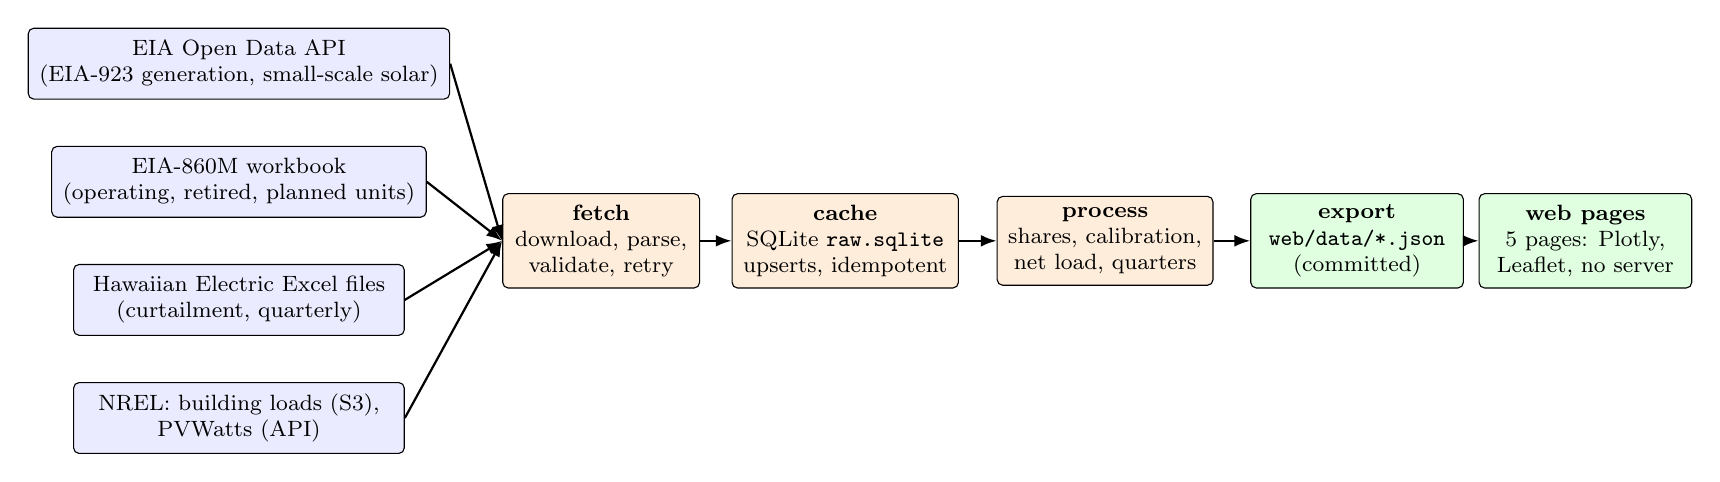
\begin{tikzpicture}[
  box/.style={draw, rounded corners=2pt, align=center, minimum height=9mm, font=\footnotesize, inner sep=4pt},
    src/.style={box, fill=blue!8, minimum width=42mm},
  stage/.style={box, fill=orange!14, minimum width=25mm},
  outbox/.style={box, fill=green!12, minimum width=27mm},
  arr/.style={-{Latex[length=2mm]}, thick}
]
\node[src] (eia)  at (0,0)    {EIA Open Data API\\(EIA-923 generation, small-scale solar)};
\node[src] (e860) at (0,-1.5) {EIA-860M workbook\\(operating, retired, planned units)};
\node[src] (heco) at (0,-3.0) {Hawaiian Electric Excel files\\(curtailment, quarterly)};
\node[src] (nrel) at (0,-4.5) {NREL: building loads (S3),\\PVWatts (API)};
\node[stage] (fetch) at (4.6,-2.25) {\textbf{fetch}\\download, parse,\\validate, retry};
\node[stage] (cache) at (7.7,-2.25) {\textbf{cache}\\SQLite \texttt{raw.sqlite}\\upserts, idempotent};
\node[stage] (proc)  at (11.0,-2.25) {\textbf{process}\\shares, calibration,\\net load, quarters};
\node[outbox] (json) at (14.2,-2.25) {\textbf{export}\\\texttt{web/data/*.json}\\(committed)};
\node[outbox] (web)  at (17.1,-2.25) {\textbf{web pages}\\5 pages: Plotly,\\Leaflet, no server};
\foreach \s in {eia,e860,heco,nrel}{\draw[arr] (\s.east) -- (fetch.west);}
\draw[arr] (fetch) -- (cache);
\draw[arr] (cache) -- (proc);
\draw[arr] (proc) -- (json);
\draw[arr] (json) -- (web);
\end{tikzpicture}}
\caption{Data flow. Each arrow is a separate module; the cache lets the process stage re-run offline. The battery
simulation has no pipeline of its own: it runs client-side on the modeled JSON.}
\label{fig:pipeline}
\end{figure}

\subsection{Modules}
\begin{itemize}
\item \textbf{Fetch} (\code{pipeline/fetch*.py}). One module per source. They download, retry on transient
 errors, and \emph{validate what came back}. Examples of why this matters: EIA answers a request for a
 not-yet-published monthly workbook with a normal-looking HTML page and a ``200 OK'' status, so the fetcher
 checks that the bytes are a real Excel (zip) file; Hawaiian Electric's Excel files are made for people, so
 rows are found by their labels rather than fixed cell positions, and the fetcher stops with a clear
 error if the layout changes rather than reading the wrong cells.
\item \textbf{Cache} (\code{pipeline/cache.py}). SQLite tables named \code{raw_*} hold exactly what was downloaded.
 Rows are upserted on a natural key, so re-running never duplicates. Derived numbers are never stored here.
\item \textbf{Process} (\code{pipeline/process*.py}). Pure functions: rows in, dictionaries out. No network, files
 or database, so they are unit-tested directly.
\item \textbf{Export} (\code{pipeline/export*.py}). Writes the JSON the pages read and stamps it with a generation
 time, source description, and kind (reported or modeled).
\item \textbf{Web} (\code{web/}). Static HTML, CSS and JavaScript modules. Plotly draws the charts and Leaflet
 (with OpenStreetMap tiles \cite{osm}) draws the map. There is no build step and no server-side code: the pages can be
 hosted on any static host, and the only network calls at view time are the JSON files, the chart libraries and
 the map tiles.
\end{itemize}

\subsection{Testing}
The repository has three layers of automated tests. 109 Python tests cover fetch parsing (including the quirks
of the real files), cache idempotence, every calculation, corrections, and the hand-written milestone file (whose
EIA-derived dates are checked against the generated plant data). 13 JavaScript tests (run with Node) test the
battery optimizer directly: power and energy limits are never exceeded, energy is conserved through the
efficiency losses, a flat day is left alone, a larger battery is never worse, and it runs in tens of
milliseconds. A headless-browser suite drives the real pages through the Chrome DevTools Protocol: it clicks the
buttons, drags the sliders, hovers and clicks on chart points with a real mouse, and checks the layout at phone
width. The browser suite caught real bugs that screenshots had not, for example the ``5y'' and ``10y'' zoom
buttons showing the wrong years because Plotly had padded the time axis.

% =========================================================================================================
\section{The data sources in detail}
\label{sec:sources}

\begin{table}[htbp]
\centering\footnotesize
\begin{tabularx}{\textwidth}{@{}>{\raggedright\arraybackslash}p{2.5cm}>{\raggedright\arraybackslash}p{3.3cm}>{\raggedright\arraybackslash}p{2.5cm}>{\raggedright\arraybackslash}p{2.3cm}X@{}}
\toprule
Source & What it measures & Resolution & Freshness & Main limits \\
\midrule
EIA Form EIA-923 (via the EIA Open Data API, route \code{electricity/facility-fuel}) &
 Net generation and fuel by plant and fuel type, in MWh &
 Monthly (about 3,000 U.S.\ plants); annual only for about 9,500 smaller plants &
 About 2--3 months behind; final figures about a year later &
 Plants of 1~MW or more only; recent months are ``provisional'' because annual-only plants report late; no hourly data \\
\addlinespace
EIA small-scale solar estimate (API route \texttt{electric-power-\allowbreak operational-data}) &
 EIA's \emph{estimate} of generation from solar systems under 1~MW, mostly rooftop &
 Monthly, statewide, from 2014 &
 A few months behind &
 Whole state of \Hawaii, not \Oahu; an estimate from utility net-metering reports, not a meter reading \\
\addlinespace
EIA-860 / EIA-860M (Excel; Operating, Retired and Planned sheets) &
 The inventory of generating units: size, fuel, technology, location, in-service and retirement month; storage energy (MWh); planned units with expected month &
 One row per generator; monthly file &
 Monthly, about a month behind &
 Plants $\geq$1~MW total and grid-connected; retirements listed only from 2002; storage energy occasionally implausible; planned dates are the developers' expectations \\
\addlinespace
Hawaiian Electric curtailment workbooks (Key Performance Metrics) &
 Delivered and curtailed wind plus utility-scale solar energy by island, and (since mid-2015) curtailed energy by reason &
 Quarterly, from Q1 2012 &
 Quarterly; past values are sometimes corrected &
 Wind and solar combined; no hour or site detail; the definition of each reason is not published with the data \\
\addlinespace
NREL End-Use Load Profiles (ResStock, ComStock; public S3 bucket) &
 Simulated electricity use of homes and businesses, and simulated output of rooftop panels on homes &
 15-minute, using actual 2018 weather &
 A fixed simulated year &
 A model, not a meter reading; time-stamped in Eastern Standard Time (5 hours off from \Hawaii); homes are statewide files, businesses are by county \\
\addlinespace
NREL PVWatts v8 (API) &
 Hourly output of a reference solar farm at a given location, in a typical meteorological year &
 Hourly &
 Static &
 A typical year, not 2024 weather; only the daily \emph{shape} is used \\
\bottomrule
\end{tabularx}
\caption{Data sources, what they measure and their limits. All are public and free; only the EIA and NREL APIs
need a (free) key.}
\label{tab:sources}
\end{table}

\subsection{EIA-923: what each plant generated}
The core of Tier~1 is the generation reported by power plants to EIA on Form EIA-923 \cite{eia923}, read through
EIA's Open Data API \cite{eia-api}. A \emph{region} is
defined as a list of plants, because EIA does not publish a fuel mix per utility or island, only per plant.
The 38 plants listed in the configuration form the \Oahu\ definition; they were found by matching EIA's plant
registry by county (Honolulu County is the island of \Oahu) and include independent power producers selling to Hawaiian Electric,
plus retired plants (Honolulu, AES Hawai\okina i) so that the history is complete. Two more plants in the same county, refinery
cogeneration plants (Tesoro/Par Hawai\okina i and Hawaii Cogen), are excluded, with the reason recorded in the
configuration, because they power the refinery rather than the grid.

EIA publishes each plant's numbers several overlapping ways (a plant total, a per-fuel breakdown, a
per-fuel-and-engine-type breakdown). The pipeline requests only the per-fuel level and drops plant-total rows so
nothing is counted twice. Battery charging appears in the data as negative generation from the fuel code for
storage, and is excluded from the totals because storage is not generation.

\paragraph{Provisional months.} About a dozen small \Oahu\ plants (mostly solar farms) report to EIA only once a
year. Until they do, the most recent months are missing their output and read low---by roughly 1 to 1.5
percentage points in recent years. The pipeline detects the last month for which the annual reporters' data
exists (their data ends in a December cluster) and marks later months \code{provisional}; the chart shades them and the
table labels them ``preliminary''. Once EIA publishes the missing year the next run corrects the numbers by
itself. For the current refresh, data are final through December 2024, so all of 2025 and 2026 are
preliminary, and the 2025 renewable-share figures in this report carry that caveat.

\subsection{The rooftop-solar estimate and how it is anchored to Hawaiian Electric}
EIA-923 does not cover rooftop panels, so the solid line in Tier~1 understates renewables. EIA publishes its own
estimate of small-scale solar generation, but for the whole state and only from 2014. The dotted line brings it
down to \Oahu. An earlier version multiplied the state figure by a fixed 77\%, the ratio of Hawaiian Electric's
reported 2024 customer-owned generation on \Oahu\ (1,211~GWh) to EIA's estimate for the state (1,573~GWh). But the
measured ratio varies from about 0.65 (2017) to 0.83 (2022), so a constant would be off by up to roughly 18\% in
some years. The current method anchors each quarter to Hawaiian Electric's own reported \Oahu\ total:
\begin{equation}
R_m \;=\; C_q\,\frac{S_m}{\sum_{m'\in q} S_{m'}}\qquad (m \in q),
\end{equation}
where $S_m$ is EIA's statewide small-scale solar estimate for month $m$, $C_q$ is Hawaiian Electric's reported
customer-owned generation for the quarter $q$ containing $m$, and $R_m$ is the resulting \Oahu\ estimate. Each
quarter therefore adds up exactly to the utility's number (this was checked for all 50 quarters), and the state
series decides only how a quarter is split across its three months. Where a quarter has not been reported, or
the state quarter is incomplete, the fixed 77\% share is used and the record's \code{rooftop_basis} field says
``assumed''; in the current data all 150 months with an estimate are ``measured''. Because rooftop energy is
added to both the numerator and the denominator, the dotted line is
\begin{equation}
s^{+}_m \;=\; 100\,\frac{E^{\text{ren}}_m + R_m}{E^{\text{tot}}_m + R_m},
\end{equation}
the share of \emph{all} electricity used, not just what utility-scale plants generated. The two lines
therefore measure different things and are labeled as such. Adding the dotted line changed no existing
number (a before/after comparison of the JSON confirmed this).

\subsection{EIA-860M: the plant inventory}
Form EIA-860 \cite{eia860} is EIA's inventory of the country's power plants. A plant must report if two conditions hold:
its generators sum to at least 1~MW of nameplate capacity, and it is connected to the local or regional electric
grid. The plant's operator files it, annually with a monthly update (EIA-860M). For each generator it records
capacity, fuel, technology, location, in-service month, retirement month (once retired), and for batteries the
energy capacity. This gives three uses in the project: the plant map, the battery fleet used as the Tier~4
default, and the planned-unit view.

What it \emph{cannot} tell us matters as much. Rooftop and other small systems are absent; generators not
connected to the grid are absent; and EIA's monthly file lists retirements only from 2002, so a plant that closed
earlier does not appear at all. That is why the map shows a single unit in 1947 (a Waiau unit retired in 2024,
the only unit from that era EIA still lists), and why the 1980s Kahuku wind turbines, the last of which shut down in
1996, are not shown. The page explains this in a collapsed explainer rather than adding data by hand, because the
requirement was ``EIA-860 plants only''.

\paragraph{A documented correction.} EIA lists the 36~MW battery at Waiawa Solar Power Hybrid as storing 4.6~MWh
(a maximum discharge of about 2.3~MW), which is not plausible; its developer reports 144~MWh
\cite{clearway}. The configuration file records this correction with its source and a guard: it applies only while
EIA still publishes exactly 4.6, so if EIA revises the value the pipeline warns rather than overriding a
possibly correct number. The exported JSON keeps both the value as filed and the value used. The correction
changes the fleet's stored energy from 985.5 to 1,124.9~MWh.

\paragraph{Planned units.} The Planned sheet lists units whose operators have told EIA they intend to build them,
with an expected in-service month and a stage from ``under construction, more than 50 percent complete'' to
``planned, regulatory approvals not initiated''. For \Oahu, it lists 18 units at five plants; the furthest is
Puuloa Energy (eleven 9.4~MW waste-biomass units, 103~MW, expected April 2029, at the earliest stage of
approval). The map treats them as planned, never as in service. Two facts limit this view: expected dates are
the developers' and often slip, and EIA lists \emph{no planned retirements} for \Oahu, so the future view can only
add plants, never remove one.

\subsection{Hawaiian Electric's curtailment files}
\label{sec:tier3}
Hawaiian Electric publishes two Excel files: delivered versus curtailed energy per island and quarter (from Q1
2012), and curtailed energy by reason (from July 2015). The original plan for Tier~3 was to \emph{estimate}
curtailment by comparing a modeled ``potential'' solar output with actual generation. That was abandoned because
the utility publishes the measured figures, and because since 2015 curtailment has been only 1--7\% of potential
a year, smaller than the uncertainties in the inputs a model would need (DC-to-AC capacity ratio, actual versus
typical weather, panel aging). A modeled estimate could not have resolved what is measured directly. (This is
reasoning, not a tested result; the modeled version was not built.)

\paragraph{Reading the files.} ``Delivered'' plus ``curtailed'' is ``potential'': what the plants could have
supplied. The categories are wind and utility-scale solar \emph{together} (``curtailable renewable
resources''), so the page cannot say how much was solar. Rooftop solar is not curtailable and is not part of
potential. Annual totals are sums of the quarters. Two internal inconsistencies are worth reporting: Hawaiian
Electric's own annual figures differ slightly from the quarter sums for a few years after corrections described
in its notes, and the two files disagree with each other in places: the by-reason columns sum to about 1.0~GWh
\emph{more} than the totals file in 2018 (6.40 versus 5.40~GWh) and about 1.5~GWh more in 2023 (23.98 versus
22.49~GWh). The pipeline reports totals from the totals file and reason amounts from the by-reason file, and marks a
year's reason breakdown as complete only when the reasons cover the whole year; the ``95\%'' headline for 2025 is
the system-constraint amount divided by the totals file's curtailed energy.

\subsection{NREL building-load and solar-shape data}
No public hourly grid data for \Hawaii\ exists that we could find: EIA's Hourly Electric Grid Monitor
covers the Lower 48 \cite{gridmonitor} and Hawaiian Electric publishes monthly and annual summaries. Tier~2 is
therefore modeled: hourly \emph{shapes} come from NREL simulations \cite{nrel-eulp,pvwatts}, and hourly \emph{sizes} are calibrated to the
real monthly EIA data. Two technical gotchas are worth recording because they would have silently corrupted every
curve. NREL's load files are stamped in Eastern Standard Time (UTC$-5$) rather than \Hawaii\ time (UTC$-10$), and
each stamp marks the \emph{end} of a 15-minute interval; the fetcher shifts them 5 hours earlier, and a test
guards this---without it the ``belly'' would land at the wrong time of day. Second, residential load files are
available only statewide, so \Oahu's share of homes (0.70, approximated from its share of the population in the
2020 Census) sets the residential part of demand.

% =========================================================================================================
\section{Methods by tier}
\label{sec:methods}

\subsection{Tier 1: renewable share}
For each month, with $g_{p,f,m}$ the generation of plant $p$ from fuel $f$:
\begin{equation}
E^{\text{tot}}_m=\sum_{p}\sum_{f\notin\text{storage}} g_{p,f,m},\qquad
E^{\text{ren}}_m=\sum_{p}\sum_{f\in\{\text{solar},\,\text{wind}\}} g_{p,f,m},\qquad
s_m=100\,\frac{E^{\text{ren}}_m}{E^{\text{tot}}_m}.
\end{equation}
Only solar and wind count as renewable (a project definition); waste-to-energy (H-POWER) and biomass do not.
This is narrower than EIA's own ``renewable'' category and than the statutory definition used for
\Hawaii's renewable portfolio standard, so the percentages here are \emph{not} compliance figures. The JSON also
keeps generation by every fuel each month so that other views can reuse it.

\subsection{Tier 2: the modeled typical day}
Let $h$ be the hour and $m$ a month of the reference year (the latest year of final Tier~1 data; 2024). Each
component has an hourly \emph{shape} $f^{(c)}_{m,h}$ from NREL and a monthly \emph{size} $M^{(c)}_m$ (MWh)
from EIA, and the hourly series is $x^{(c)}_{m,h} = M^{(c)}_m\,f^{(c)}_{m,h}/\sum_h f^{(c)}_{m,h}$. The
components and their sizes are: utility solar (PVWatts shape; size from EIA-923 solar), wind (flat shape; size from
EIA-923 wind), rooftop solar (ResStock shape; size $R_m$ as in Section~\ref{sec:sources}, using the fixed
77\% share for the reference year, where it is exact) and customer demand (ResStock plus ComStock shape; size
equal to \Oahu's generation plus rooftop solar, i.e.\ an energy balance ignoring losses and imports). In megawatts,
hour by hour:
\begin{align}
\text{grid load}_h &= \text{customer demand}_h - \text{rooftop}_h && \text{(what the utility ``sees'')}\\
\text{net load}_h &= \text{grid load}_h - \text{utility solar}_h - \text{wind}_h && \text{(what fuel-burning plants supply)}
\end{align}
A ``typical weekday'' in each season is the hourly average of that season's Monday--Friday days (64--66
weekdays per season). Four headline numbers are computed from the net-load curve: the midday low (minimum over 9~AM
to 3~PM), the evening peak (maximum after it), the climb between them, and the steepest three-hour ramp.

\begin{table}[htbp]
\centering\small\setlength{\tabcolsep}{4pt}
\begin{tabular}{@{}lrrrr@{}}
\toprule
Season (weekday average) & Midday low & Evening peak & Climb & 3\,h ramp\\
\midrule
Winter (Dec--Feb) & 490 & 1,072 & +582 & +414\\
Spring (Mar--May) & 387 & 993 & +606 & +397\\
Summer (Jun--Aug) & 460 & 1,017 & +557 & +376\\
Fall (Sep--Nov) & 538 & 1,064 & +526 & +359\\
\bottomrule
\end{tabular}
\caption{Modeled net-load statistics for a typical weekday, reference year 2024, all in MW (``3\,h ramp'' is the
steepest three-hour ramp). The midday low is at noon and the peak at 6~PM in every season; the steepest ramp starts at 2~PM.}
\label{tab:duck}
\end{table}

\paragraph{Validation, honestly.} What could be checked, and what could not:
\begin{itemize}
\item \emph{Rooftop total.} The model's rooftop energy for 2024 (1,211~GWh) equals Hawaiian Electric's reported
 figure. This is agreement \emph{by construction}, since the 77\% share was derived from that same figure; it
 checks the arithmetic, not the model.
\item \emph{Evening peak (an independent check).} Hawaiian Electric told the \Hawaii\ Public Utilities Commission
 that \Oahu's 2020 system peak was 1,087~MW at 5:26~PM, with 2010--2019 peaks between 1,141 and 1,206~MW
 \cite{adequacy}. The modeled average weekday peaks at 993--1,072~MW around 6~PM, depending on season: the right
 size and nearly the right hour, and, as expected, a little below the single busiest day.
\item \emph{Delivered energy.} Hawaiian Electric's ``delivered'' wind plus solar is 0.85--0.94 of EIA's solar plus wind
 for 2021--2024. The two count slightly different plant sets, so exact equality is not expected; a stable ratio
 near one shows that both describe the same quantity.
\item \emph{Not checked.} The overnight and midday minima, for which no public figures were found. The modeled overnight
 grid load (roughly 40--50\% of the evening peak) looks lower than would be expected for \Oahu, which exaggerates
 how deep the belly looks relative to the night.
\item \emph{Not modeled.} Curtailment, so the true midday dip is probably shallower than drawn.
\end{itemize}
Structurally, the chart combines 2018 weather shapes with 2024 sizes, uses one average weekday per season (which
smooths out cloudy and clear days), and leaves out weekends. It illustrates the pattern; it does not record any day.

\subsection{Tier 3: curtailment}
No modeling is involved. The pipeline reads the two workbooks, locates \Oahu's section by label, and computes
$\text{potential}=\text{delivered}+\text{curtailed}$ and $\text{curtailment \%}=100\,\text{curtailed}/\text{potential}$
for each quarter and year, with reasons where available. Cross-checks against Tier~1 (the ratio above) and
against EIA's rooftop estimate (which fixed the 77\% share) are printed on every run.

\subsection{Tier 4: the battery simulation}
For a 24-hour net-load curve $n_h$, battery power limit $P$, energy capacity $B$ and round-trip efficiency $\eta$
(split evenly, $\sqrt{\eta}$ each way), the browser chooses a charge/discharge schedule to minimize, over a run of
$T=120$ hours (the same day repeated five times),
\begin{equation}
\sum_{t=1}^{T}\Bigl[\max(r_t,\,F)^{2} + \lambda\,\text{curt}_t + \epsilon\,(c_t+d_t)\Bigr],\qquad
r_t=n_t+c_t-d_t,\quad \text{curt}_t=\max(0,\;F-r_t),
\end{equation}
where $c_t$ and $d_t$ are the power drawn from and delivered to the grid, subject to $c_t,d_t\le P$ and a state of
charge kept in $[0,B]$; $F$ is the ``fossil minimum output'' floor; $\lambda = 4\max(F,\max_h n_h)+1$ is a penalty
large enough that absorbing one MW of surplus always beats any flattening it could buy; and $\epsilon=0.01$ is a
tiny throughput penalty that only breaks ties. The squared term models fossil plants becoming costlier per MWh as
they are pushed harder, so minimizing it flattens the day. It is solved exactly by dynamic programming over a
200-level state-of-charge grid, with perfect foresight. The battery starts \emph{empty} and the third of the five
days is shown, so the display is a steady-state day. (Starting with a free charge was tried first and was wrong:
the optimizer simply spent the gift slowly, so the ``typical day'' was a draining day. A test now guards this.)

The sliders are battery power (default 326~MW, the island's fleet), energy (1,125~MWh), efficiency (85\%), extra
utility-scale solar (0\%) and the fossil minimum ($F=300$~MW). The last is an \textbf{invented illustration}: no public figure
for how low \Oahu's fossil units can be turned down was found; 300~MW was chosen so today's typical weekday is not
curtailed while extra solar visibly is, and it is labeled ``illustrative'' on the page.

\begin{table}[htbp]
\centering\small\setlength{\tabcolsep}{4pt}
\begin{tabular}{@{}lrrr@{}}
\toprule
Spring weekday, MW & Evening peak & Midday low & 3\,h ramp\\
\midrule
No battery & 993 & 387 & +397\\
Kapolei alone (185\,MW / 565\,MWh) & 808 & --- & ---\\
Whole fleet (326\,MW / 1,125\,MWh) & 687 & 557 & +129\\
\bottomrule
\end{tabular}
\caption{Simulated effect of storage on the modeled spring weekday. The fleet result assumes the whole fleet
may charge from the grid at will, which is an upper bound (batteries paired with solar farms may be restricted).}
\end{table}

\paragraph{What this simulation gets right and wrong.} It models load shifting only. It does not model frequency
response, synthetic inertia or black start; battery aging; reserves; market rules; weekends; demand response; line
limits; or changes to rooftop solar. It also models only one kind of curtailment (oversupply against a floor),
whereas Tier~3 shows that most recent curtailment is classified as system constraint, so it may
\emph{understate} what real batteries do. The optimizer also cycles the battery overnight (minimizing squared
net load flattens the whole day), and energy stored outside solar hours comes from fossil plants, so it is not free.

% =========================================================================================================
\section{What the visualizations show}
\label{sec:results}

\subsection{Renewable share over time}
Table~\ref{tab:annual} and Figure~\ref{fig:share} summarize Tier~1. The utility-scale share is zero for a
decade, steps up with Kahuku Wind (2011), climbs slowly with small solar and Kawailoa Wind, then jumps in
2020, the first full year of the four solar farms that started in late 2019 (about 130~MW; a smaller total in the
pandemic year also lifts the ratio slightly). It plateaus at 11--12\% from 2023. The estimate that includes rooftop solar tells a different story: it starts
at 8.1\% in 2014 and reaches 26.6\% in 2025, because rooftop generation grew from an estimated 399 to
1,336~GWh a year. Roughly two thirds of the solar and wind electricity used on \Oahu\ in 2025 (about 1,336 of 2,041~GWh) is thus rooftop
solar, invisible to the plant-level survey, which is the main reason the site shows both lines.

\begin{table}[htbp]
\centering\small\setlength{\tabcolsep}{4pt}
\begin{tabular}{@{}lrrrrr@{}}
\toprule
Year & Total (GWh) & Solar+wind (GWh) & Share (\%) & Rooftop (GWh) & Share incl.\ rooftop (\%)\\
\midrule
2005 & 8,163 & 0 & 0.0 & --- & ---\\
2011 & 7,359 & 59 & 0.8 & --- & ---\\
2014 & 7,109 & 208 & 2.9 & 399 & 8.1\\
2017 & 6,834 & 283 & 4.1 & 634 & 12.3\\
2019 & 6,779 & 298 & 4.4 & 881 & 15.4\\
2020 & 6,434 & 544 & 8.5 & 957 & 20.3\\
2022 & 6,440 & 655 & 10.2 & 1,101 & 23.3\\
2023 & 6,387 & 768 & 12.0 & 1,139 & 25.3\\
2024 & 6,374 & 753 & 11.8 & 1,211 & 25.9\\
2025$^{*}$ & 6,331 & 705 & 11.1 & 1,336 & 26.6\\
\bottomrule
\end{tabular}
\caption{Selected annual values from the Tier~1 data. $^{*}$Preliminary (final data end in December 2024): small
annual-reporting plants are missing, so utility-scale figures read slightly low.}
\label{tab:annual}
\end{table}

\begin{figure}[!htbp]
\centering
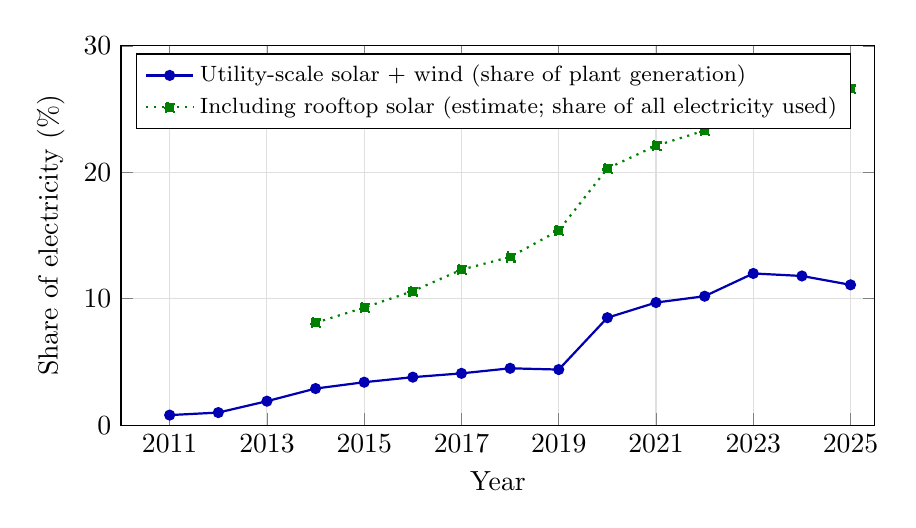
\begin{tikzpicture}
\begin{axis}[width=0.92\textwidth, height=6.4cm, xmin=2010, xmax=2025.5, ymin=0, ymax=30,
  xlabel={Year}, ylabel={Share of electricity (\%)}, xtick={2011,2013,2015,2017,2019,2021,2023,2025},
  x tick label style={/pgf/number format/1000 sep={}}, legend style={at={(0.02,0.98)}, anchor=north west, font=\footnotesize}, legend cell align=left,
  grid=major, grid style={gray!25}, every axis plot/.append style={thick}, mark size=1.6pt]
\addplot[blue!70!black, mark=*] coordinates {(2011,0.8)(2012,1.0)(2013,1.9)(2014,2.9)(2015,3.4)(2016,3.8)(2017,4.1)(2018,4.5)(2019,4.4)(2020,8.5)(2021,9.7)(2022,10.2)(2023,12.0)(2024,11.8)(2025,11.1)};
\addlegendentry{Utility-scale solar + wind (share of plant generation)}
\addplot[green!50!black, dotted, mark=square*] coordinates {(2014,8.1)(2015,9.3)(2016,10.6)(2017,12.3)(2018,13.3)(2019,15.4)(2020,20.3)(2021,22.1)(2022,23.3)(2023,25.3)(2024,25.9)(2025,26.6)};
\addlegendentry{Including rooftop solar (estimate; share of all electricity used)}
\end{axis}
\end{tikzpicture}
\caption{Annual renewable share, recomputed from the Tier~1 data (2025 preliminary). The two lines use different
denominators (see Section~\ref{sec:sources}).}
\label{fig:share}
\end{figure}

\begin{figure}[!htbp]
\centering
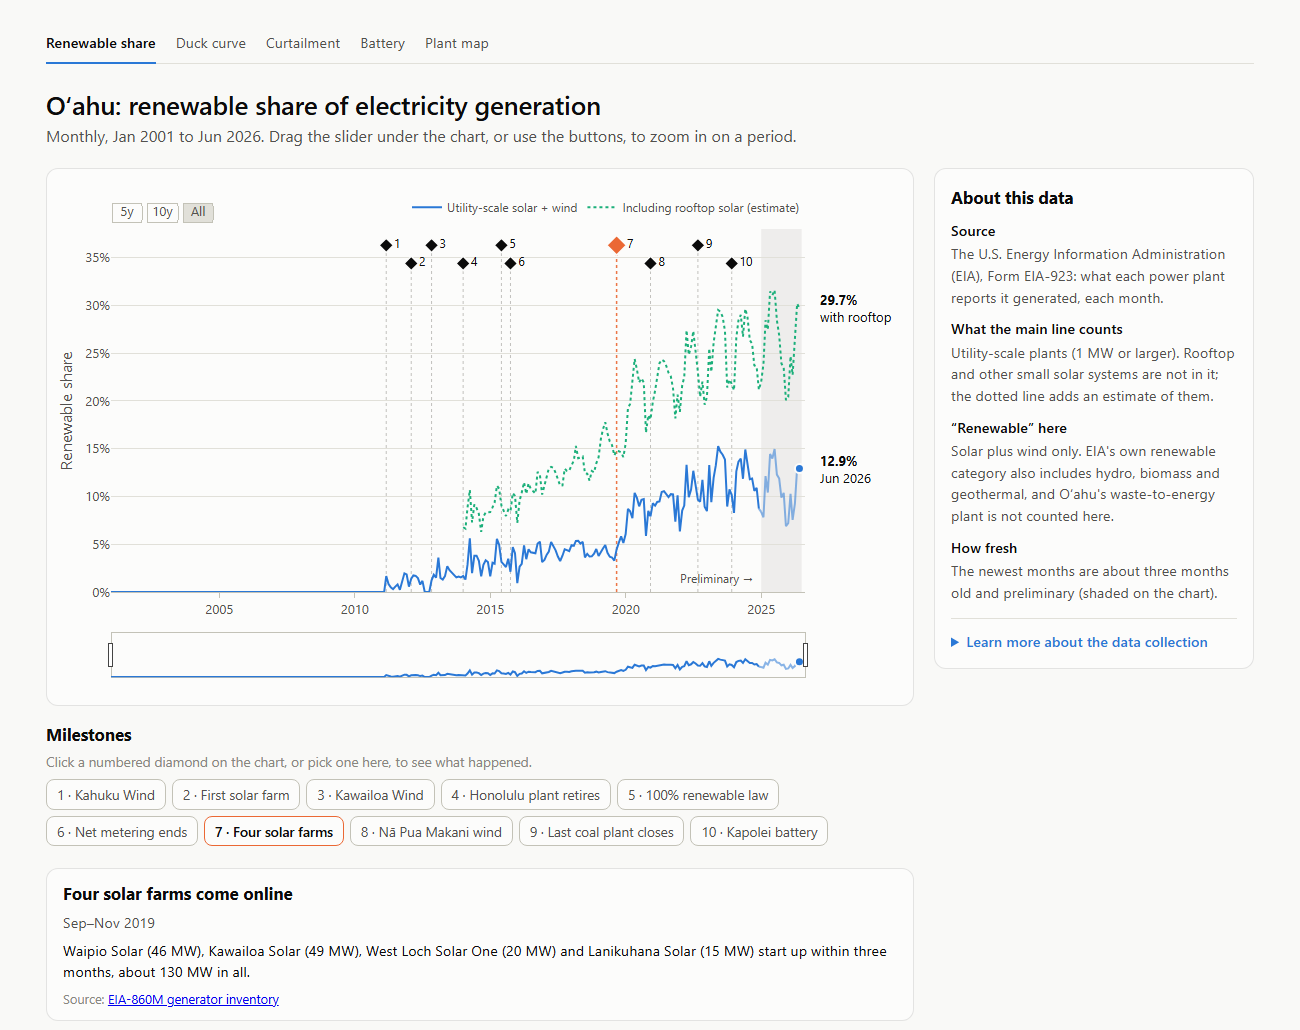
\includegraphics[width=0.95\textwidth]{figures/fig_tier1.png}
\caption{The Tier~1 page. Numbered diamonds are the ten milestones (e.g.\ 1: Kahuku Wind, March 2011; 7: four solar farms,
September--November 2019, selected here); each opens a card with a one-sentence description and a source link.
Hovering a line shows only that line's month and value.}
\label{fig:tier1}
\end{figure}

\paragraph{Fuel mix and capacity.} In 2024 (final data) the utility-scale plants generated 6,374~GWh: residual fuel
oil 5,091~GWh (79.9\%), solar 455 (7.1\%), wind 298 (4.7\%), municipal solid waste 338 (5.3\%), distillate fuel oil
174 (2.7\%) and other biomass liquids 19 (0.3\%). Nameplate capacity in service in July 2026 is dominated by oil
(1,429~MW of 2,394~MW, 60\%), while solar is 355~MW (14.8\%). Because solar's capacity factor is far below oil's
availability, a share of capacity translates into a much smaller share of energy.

\paragraph{A sanity check worth showing: implied capacity factor.} Combining the two EIA sources gives a
consistency check that the site does not currently display: generation from EIA-923 divided by nameplate capacity
in service from EIA-860M times hours.
\begin{table}[htbp]
\centering\small\setlength{\tabcolsep}{4pt}
\begin{tabular}{@{}lrrrrrr@{}}
\toprule
& 2019 & 2020 & 2022 & 2023 & 2024 & 2025$^{*}$\\
\midrule
Solar, average MW in service & 95 & 195 & 222 & 277 & 287 & 322\\
Solar, implied capacity factor (\%) & 18.2 & 20.9 & 20.9 & 20.0 & 18.0 & 16.4\\
Wind, average MW in service & 99 & 101 & 127 & 127 & 127 & 127\\
Wind, implied capacity factor (\%) & 17.0 & 20.9 & 22.5 & 25.6 & 26.8 & 21.9\\
\bottomrule
\end{tabular}
\caption{Implied capacity factors for the plants in the Tier~1 list, using each unit's nameplate (AC) capacity from
the month it enters service. $^{*}$Preliminary generation. Values of 17--27\% are plausible for \Oahu, but the
fall in solar's figure in 2024--2025 is a question the data raises, not an answer: candidate explanations
include new capacity ramping up mid-year, curtailment, weather, plant degradation, and (for 2025) missing
small-plant data. The calculation is not part of the site.}
\label{tab:cf}
\end{table}

\subsection{The modeled duck curve}
Figure~\ref{fig:duck} shows the modeled spring weekday: customer demand (dotted), grid load after rooftop solar,
and net load after utility solar and wind. The rooftop layer is the largest source of the belly; utility solar and
wind take a further bite. The evening climb of 606~MW over six hours from noon to 6~PM, with a steepest three-hour
segment of +397~MW, is the number a system operator would translate into ramping requirements. Winter has the
highest peak (1,072~MW) and fall the shallowest belly (538~MW).

\begin{figure}[!htbp]
\centering
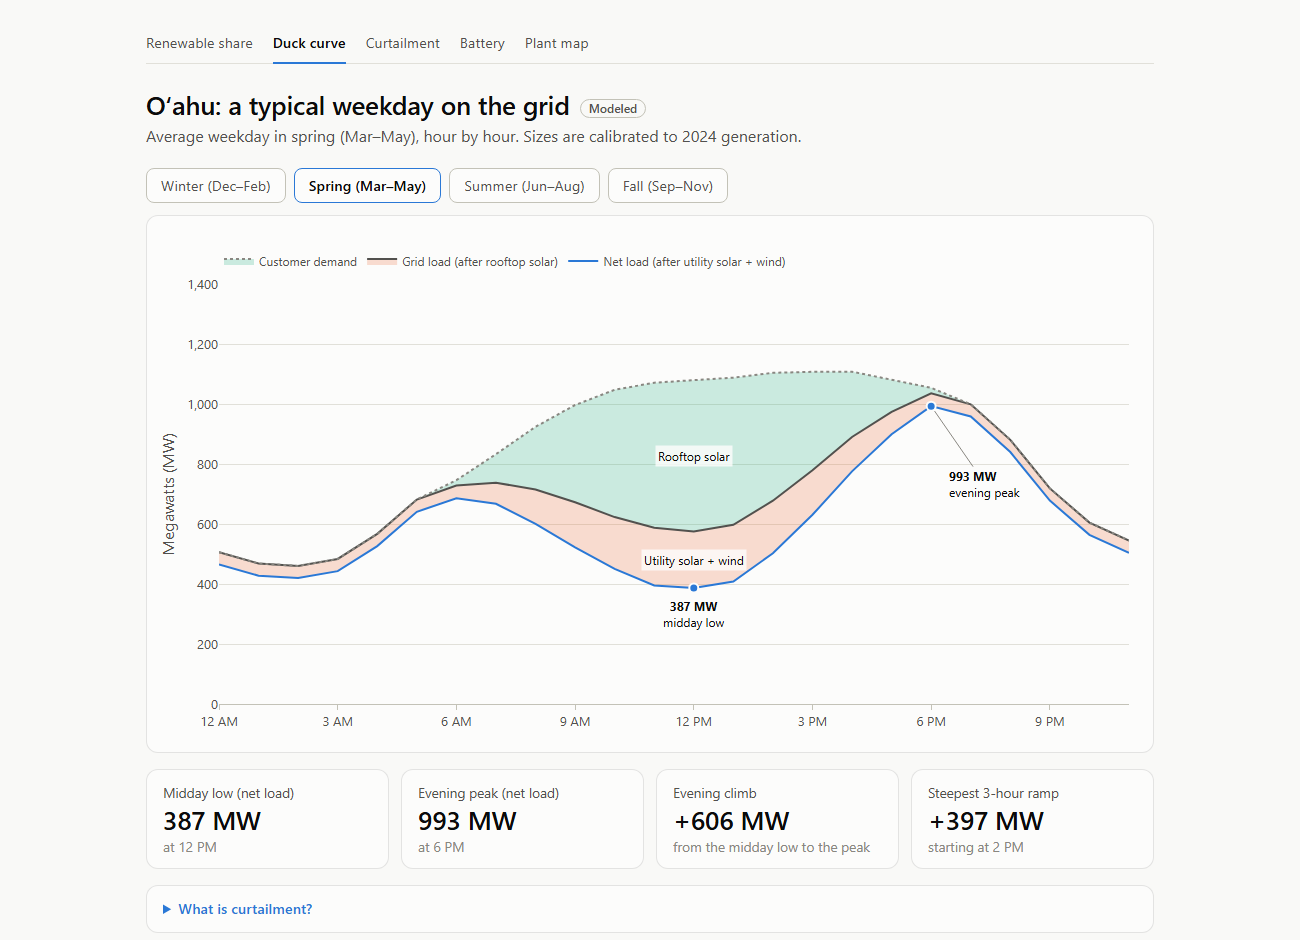
\includegraphics[width=0.88\textwidth]{figures/fig_duck.png}
\caption{The Tier~2 page (spring, modeled). The page is tagged ``Modeled'' and says in words that it is an
illustration of the pattern rather than a record of any day.}
\label{fig:duck}
\end{figure}

\subsection{Curtailment}
Curtailed wind and solar were small in energy terms but changed sharply in character. In 2012 it was 14\% of a
tiny base (Q3 2012 reached 25.7\%); it fell to 1--2.4\% from 2014 to 2019, rose to 7.1\% in 2021 and 6.6\% in 2022
as solar farms arrived, and dropped to 3.0\% (2023), 3.5\% (2024) and 1.6\% (2025). The reason breakdown
(Figure~\ref{fig:curtail}) is more revealing than the total: from 2017 to 2019 nearly all curtailment was ``system
constraint''; in 2021--2022 about half was ``oversupply''; and by 2025 oversupply had almost disappeared
(0.6 of 14.3~GWh) while system constraint stayed around 14--19~GWh. The decline of oversupply curtailment
coincides with new batteries, including Kapolei Energy Storage (December 2023), but the data alone cannot
attribute it, since demand, solar additions, dispatch practice and weather also changed. And because system
constraint is now the dominant category and Hawaiian Electric does not publish what it contains, the site
cannot say how much of it storage could relieve. (An earlier draft of the project said batteries would help only
partly; that was an overreach and was removed.)

\begin{figure}[!htbp]
\centering
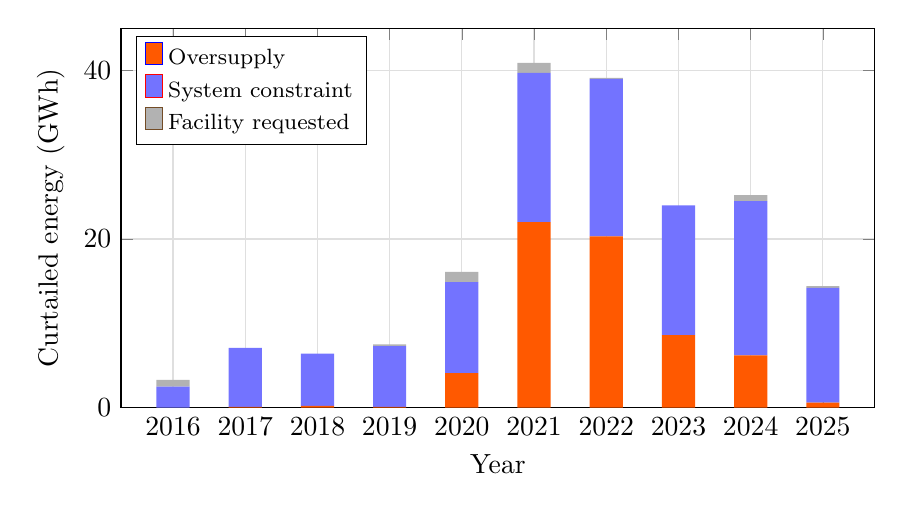
\begin{tikzpicture}
\begin{axis}[ybar stacked, width=0.92\textwidth, height=6.4cm, bar width=12pt, ymin=0, ymax=45,
  xlabel={Year}, ylabel={Curtailed energy (GWh)}, xtick=data, x tick label style={/pgf/number format/1000 sep={}},
  legend style={at={(0.02,0.98)}, anchor=north west, font=\footnotesize}, legend cell align=left, grid=major, grid style={gray!25}, enlarge x limits=0.08]
\addplot+[fill=orange!70!red, draw=none] coordinates {(2016,0.0)(2017,0.1)(2018,0.2)(2019,0.1)(2020,4.1)(2021,22.0)(2022,20.3)(2023,8.6)(2024,6.2)(2025,0.6)};
\addplot+[fill=blue!55, draw=none] coordinates {(2016,2.5)(2017,7.0)(2018,6.2)(2019,7.2)(2020,10.8)(2021,17.7)(2022,18.7)(2023,15.4)(2024,18.3)(2025,13.6)};
\addplot+[fill=gray!60, draw=none] coordinates {(2016,0.8)(2017,0.0)(2018,0.0)(2019,0.2)(2020,1.2)(2021,1.2)(2022,0.1)(2023,0.0)(2024,0.7)(2025,0.2)};
\legend{Oversupply, System constraint, Facility requested}
\end{axis}
\end{tikzpicture}
\caption{Curtailed wind and utility-scale solar on \Oahu\ by reason, from Hawaiian Electric's by-reason file
(GWh per year; 2016 is the first full year of reasons). Bars show the by-reason sums; in 2018 and 2023 these
exceed the totals file by about 1.0 and 1.5~GWh (Section~\ref{sec:sources}).}
\label{fig:curtail}
\end{figure}

\begin{figure}[!htbp]
\centering
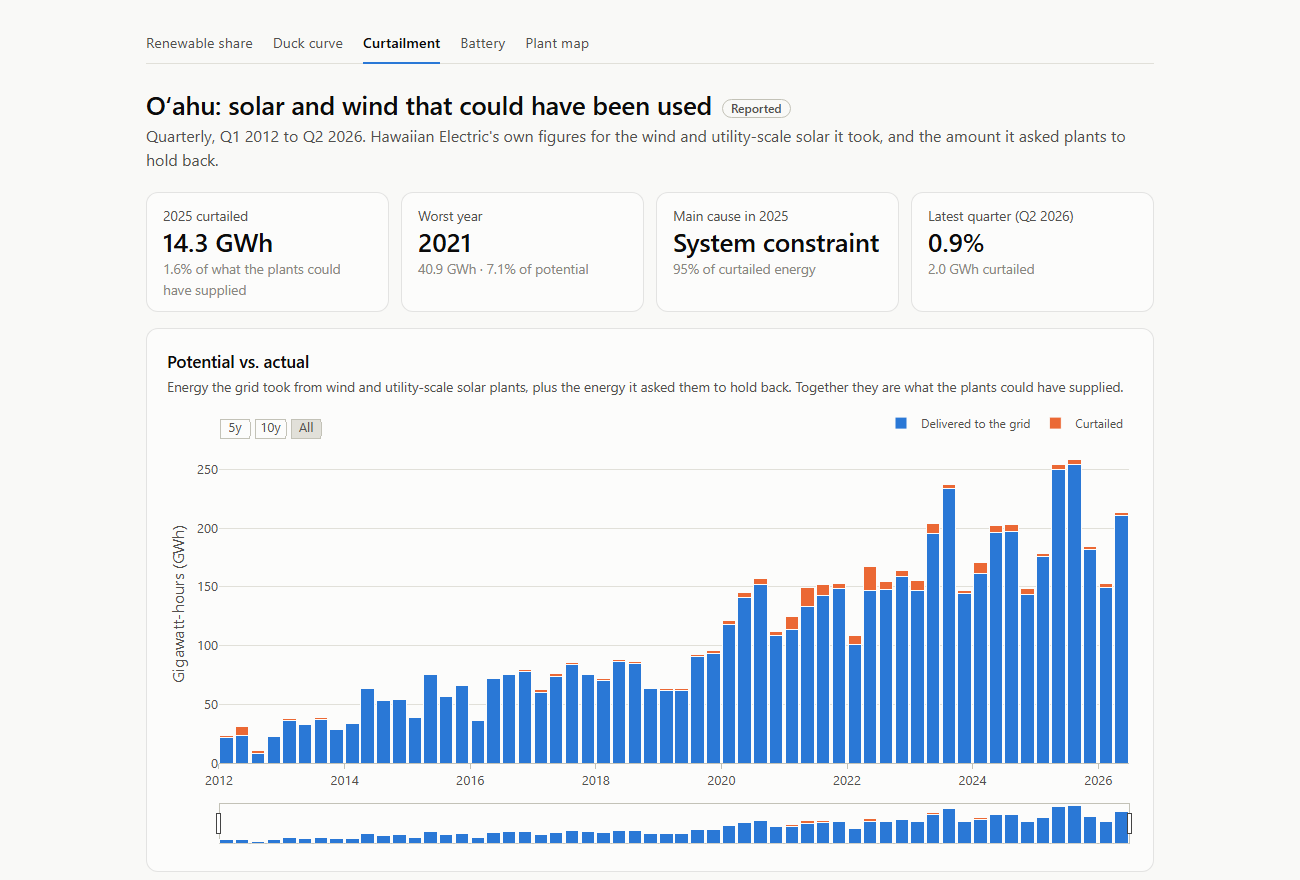
\includegraphics[width=0.9\textwidth]{figures/fig_curtailment.png}
\caption{The Tier~3 page: 2025 curtailment, worst year, main cause, latest quarter, and quarterly delivered versus
curtailed energy since 2012 (tagged ``Reported'').}
\end{figure}

\subsection{Battery simulation}
\begin{figure}[!htbp]
\centering
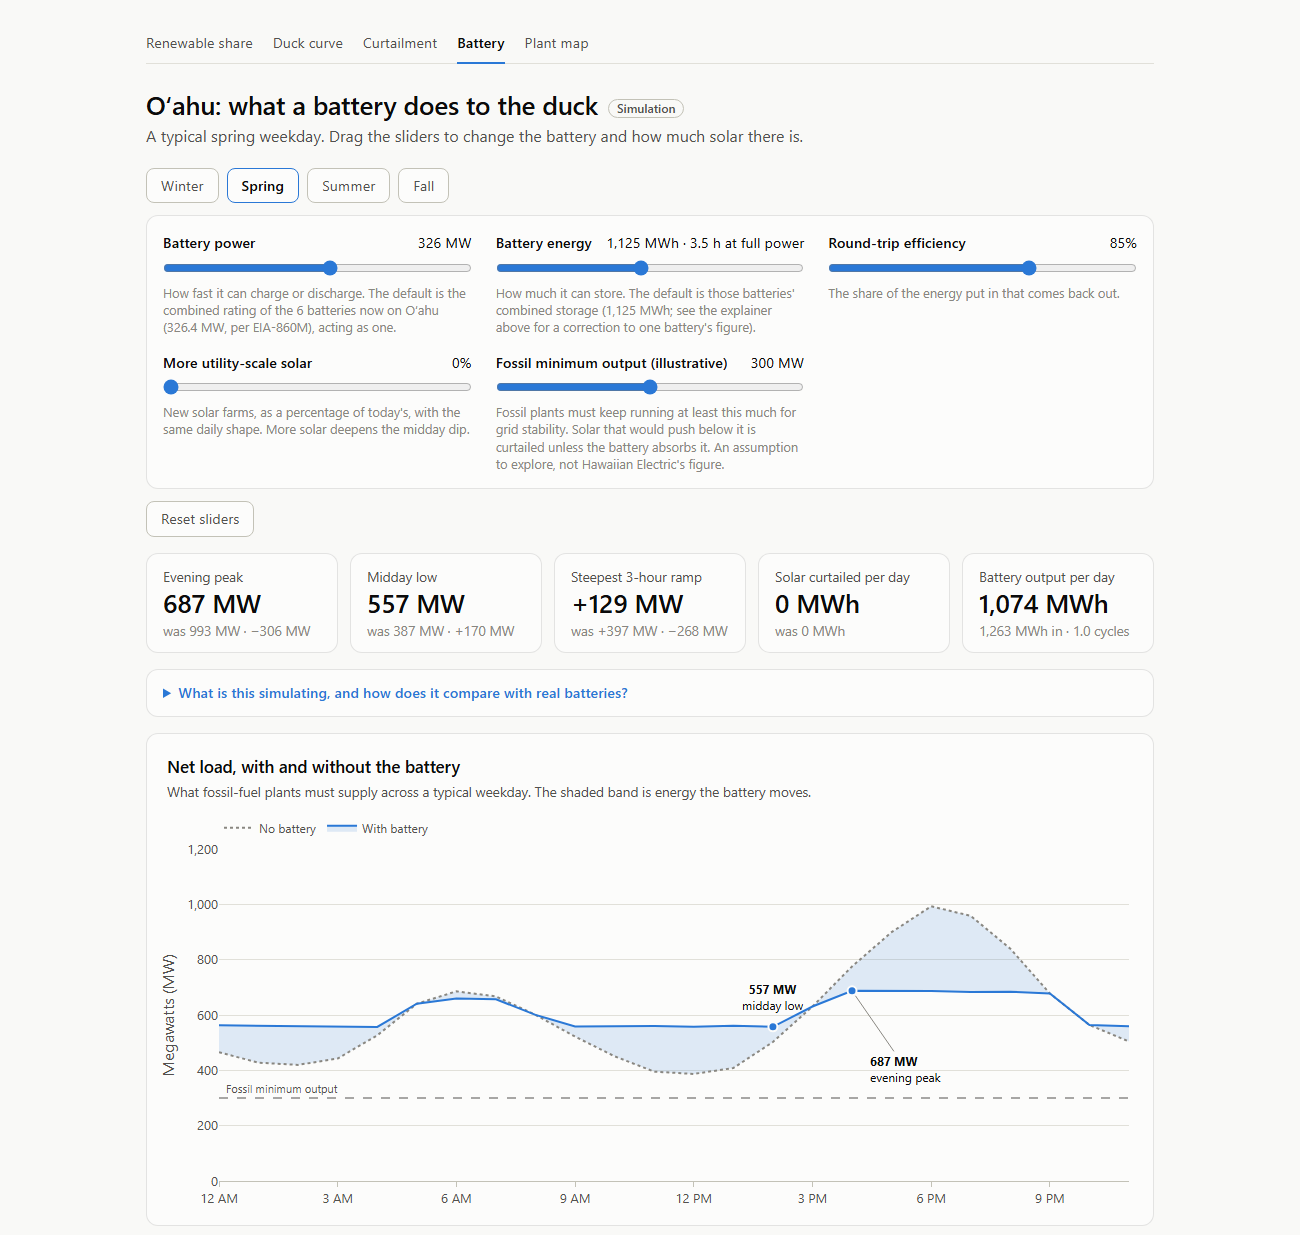
\includegraphics[width=0.8\textwidth]{figures/fig_battery.png}
\caption{The Tier~4 page (spring, default sliders). With the island's whole battery fleet acting as one battery,
the modeled evening peak falls from 993 to 687~MW and the midday low rises from 387 to 557~MW; the battery cycles
about once a day.}
\end{figure}
The simulation is best read as a demonstration of the \emph{interaction} between solar and storage rather than a
forecast. With 200\% more solar and no battery, about 783~MWh of solar a day would be curtailed against the 300~MW
floor and the fleet absorbs all of it; the effect saturates further out (at +300\% solar about 376 of 1,604~MWh/day
are still curtailed; at +400\% about 1,251 of 2,528). The real curtailed energy on the page (about 39~MWh a day on
average in 2025) is shown only for scale.

\subsection{The plant map}
The map page (Figure~\ref{fig:map}) puts each unit on a time slider from December 1947 to
April 2029; it opens on the current month, has a Today button, and Play sweeps the timeline month by month at
about 109 months per second. Circle size is capacity in service on the selected date and colour is the fuel of the
largest units; planned plants are faint circles with a dashed outline and are never counted as in service. The
side panel and list update with the slider. In August 2022 the map shows 29 plants including the 203~MW AES coal plant;
two months later the coal circle is gone, matching its retirement on 1~September.

\begin{figure}[!htbp]
\centering
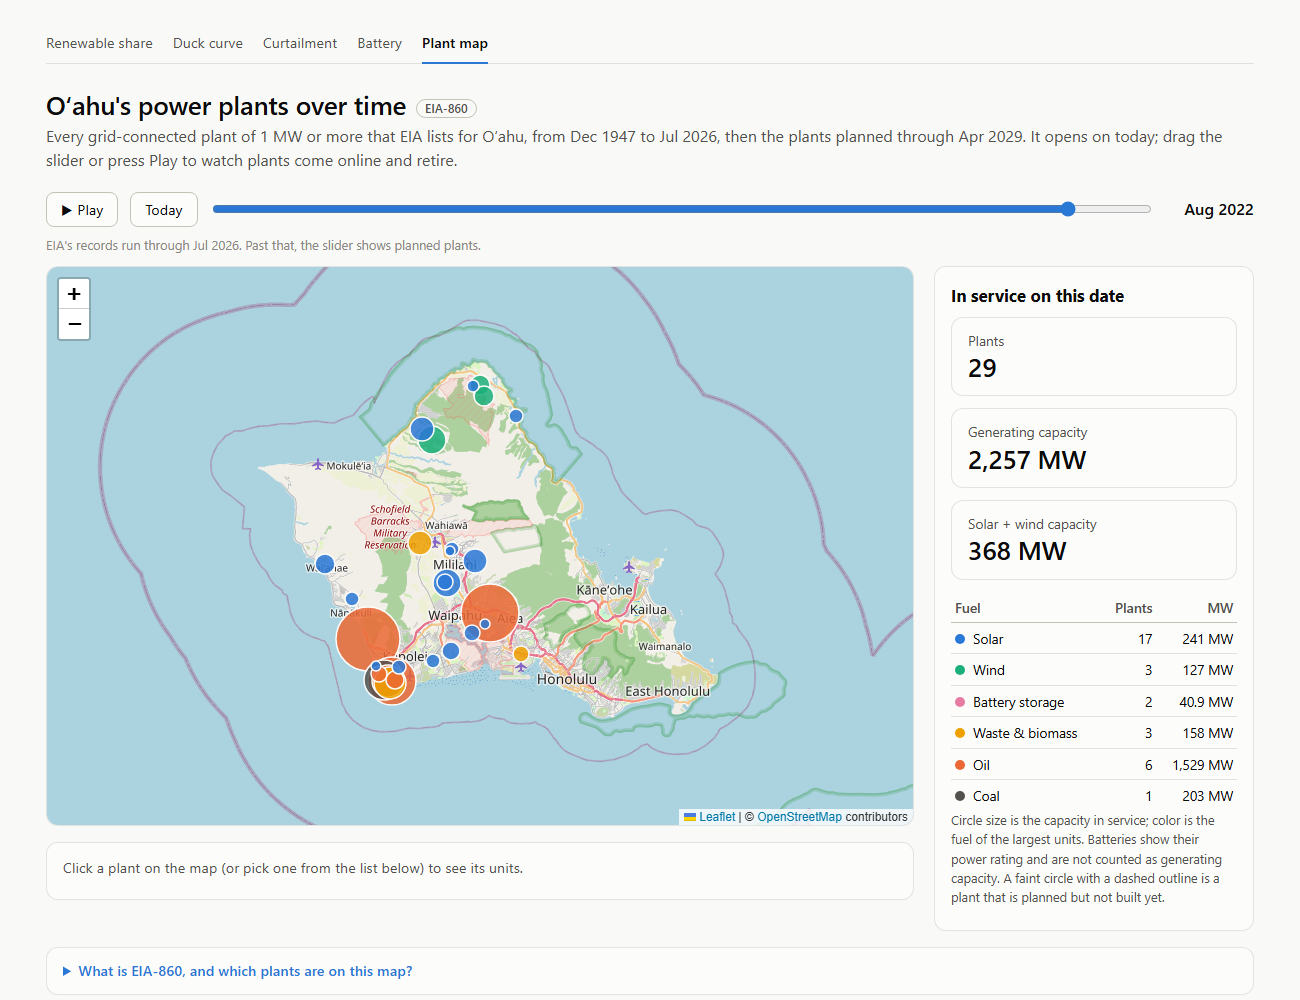
\includegraphics[width=0.49\textwidth]{figures/fig_map_2022.png}\hfill
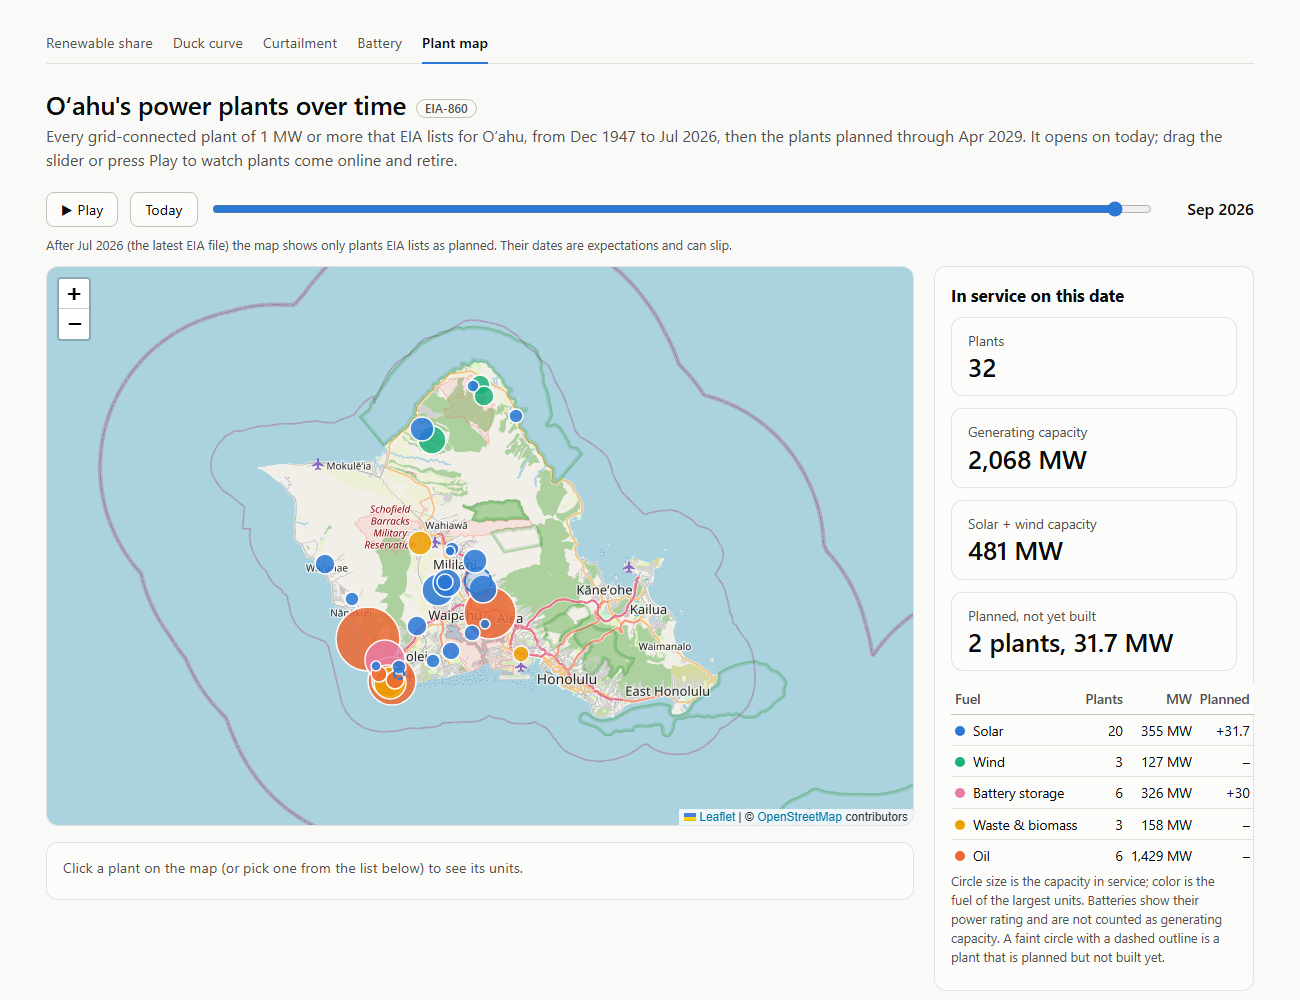
\includegraphics[width=0.49\textwidth]{figures/fig_map_today.png}
\caption{The plant map. Left: August 2022, the last month with coal (dark circle, 203~MW). Right: today's date
(September 2026); the two dashed circles are solar-plus-battery projects that EIA lists as expected in September 2026,
and the statistics count only in-service units.}
\label{fig:map}
\end{figure}

% =========================================================================================================
\needspace{12\baselineskip}
\section{Data quality, uncertainty and limitations}
\label{sec:limits}

{\footnotesize\setlength{\tabcolsep}{4pt}
\begin{longtable}{@{}>{\raggedright\arraybackslash}p{3.4cm}>{\raggedright\arraybackslash}p{5.9cm}>{\raggedright\arraybackslash}p{6.0cm}@{}}
\caption{Principal limitations, their effect and what mitigates or would fix them.}\\
\toprule
Limitation & Effect on what the charts show & Mitigation or possible fix \\
\midrule
\endfirsthead
\toprule
Limitation & Effect on what the charts show & Mitigation or possible fix \\
\midrule
\endhead
\bottomrule
\endfoot
\bottomrule
\endlastfoot
No public hourly grid data for \Hawaii & Tier~2 (and hence Tier~4) are modeled: shape from NREL simulations of 2018 weather, size from 2024 monthly totals; one average weekday per season & Labeled ``Modeled''; peak checked against HECO's filing; real utility data would replace the shapes without changing the chart \\
State-to-island scaling & Rooftop solar is estimated for the state; \Oahu's share varies 0.65--0.83 by year and the home share (0.70) is population-based & Rooftop total anchored to HECO's reported quarterly totals; 0.77 only as fallback \\
1~MW reporting threshold and 2--3 month lag (EIA-923/860) & Small plants are invisible; newest months preliminary and read low & Shaded ``preliminary'' months; automatic correction on re-run \\
Wind and solar reported together (HECO) & Cannot say how much of curtailment was solar or wind & Ask for split by technology \\
Quarterly curtailment & Nothing about when in the day it happens or at which plant & Ask for hourly or event-level data \\
Category definitions unpublished & ``System constraint'' cannot be broken down, so what storage could relieve is unknown & Ask HECO for definitions; consult the utility's curtailment reports to the regulator \\
Plant list is configuration & A new or renamed plant must be added by hand (a discovery helper exists) & Automate by county match on each EIA-860M refresh \\
Definitions of ``renewable'' & Solar plus wind only; not the state RPS definition; waste-to-energy excluded & Stated on every page; a switch in the configuration \\
Retirements listed only from 2002 & The map's early decades are sparse and survivor-biased & Explained on the page; would need a supplementary historical source \\
Modeled battery vs.\ real batteries & Load shifting only; perfect foresight; illustrative fossil minimum; no services & Labeled ``Simulation''; explainer compares with real services \\
Planned-unit dates & Operators' expectations; cancelled projects vanish from the sheet; no planned retirements listed & Caveat shown with every planned plant \\
\end{longtable}}

\subsection{How errors were guarded against}
\begin{itemize}
\item \emph{Format drift.} Fetchers locate data by labels and fail with a clear message if a layout changes;
 fake-success pages are detected by content, not status code.
\item \emph{Silent unit and time-zone errors.} Tested (the 5-hour NREL shift; quarter/month mapping; strings that
 look like numbers; three apostrophe styles in ``\Oahu'').
\item \emph{Double counting.} Nested EIA rows are dropped; battery charging is excluded from totals.
\item \emph{Guarded corrections.} Overrides apply only to the exact value they were written for and are logged in the JSON.
\item \emph{Calculation changes.} Adding the rooftop line and later re-anchoring it were verified to leave every
 existing field unchanged, by comparing the outputs before and after.
\item \emph{Claims.} Two claims made earlier in the project were withdrawn after review: a statement that batteries
 ``may not relieve'' system-constraint curtailment (unsupported), and a report of a cause for the end of the early
 Kahuku wind farm that no source confirmed.
\end{itemize}

% =========================================================================================================
\section{Additional data that would improve the visualizations}
\label{sec:extra}

The current site is limited less by design than by the resolution of public data. Table~\ref{tab:extra} lists
data that would most improve it, roughly in priority order, with the visualization it would enable and who would
benefit. ``Ask'' means the data probably exists inside the utility or the regulator's dockets and would have to be
requested or found in public filings; we have not confirmed which are already published.

{\footnotesize\setlength{\tabcolsep}{4pt}
\begin{longtable}{@{}>{\raggedright\arraybackslash}p{3.4cm}>{\raggedright\arraybackslash}p{5.9cm}>{\raggedright\arraybackslash}p{6.0cm}@{}}
\caption{Data that would most improve the visualizations, what it would add and who benefits.}\label{tab:extra}\\
\toprule
Data & What it would add & Who would find it useful, and why \\
\midrule
\endfirsthead
\toprule
Data & What it would add & Who would find it useful, and why \\
\midrule
\endhead
\bottomrule
\endfoot
\bottomrule
\endlastfoot
\textbf{1. Hourly (or 5-minute) system load and generation by unit} (utility system-operations data; ``ask'') &
 Replace the modeled duck curve with measured net load; plot real days, extremes (highest peak, deepest belly) and trends by year; validate or correct the modeled overnight and midday levels &
 Utilities and planners (communication, integration studies); regulators (evidence for dockets); researchers (calibrating models); developers (sizing storage against real ramps); educators \\
\addlinespace
\textbf{2. Curtailment by hour, plant, technology and cause}, with definitions of each reason (ask) &
 Show \emph{when} curtailment occurs, which plants bear it, and separate solar from wind; a heat-map of curtailment by hour and month; test whether oversupply falls after batteries &
 Independent power producers and lenders (revenue risk under PPA terms, which vary by contract); storage developers (where a battery earns its keep); regulators (fairness of curtailment allocation) \\
\addlinespace
\textbf{3. Metered or inverter-telemetry rooftop solar and net demand}, aggregated by hour and by circuit region (ask) &
 Replace the estimated rooftop layer; show real behind-the-meter output on clear and cloudy days; expose true customer demand; a reconciled energy balance &
 Utilities (visibility of rooftop solar is the hardest part of operating a high-DER grid); solar installers; policy analysts evaluating net-metering successor programs \\
\addlinespace
\textbf{4. Storage operations}: hourly charge, discharge and state of charge per battery, and which services it provided &
 Compare the simulation with what batteries actually do; show service use (frequency response versus shifting); estimate real round-trip efficiency and cycling &
 Storage owners and investors; system planners; researchers testing dispatch models \\
\addlinespace
\textbf{5. Customer-sited storage and flexible loads} (home batteries, grid-service programs, EV charging, water heaters) &
 Add the evening supply that customer batteries provide and the demand-side flexibility that flattens the duck; EV charging load shapes &
 Program designers; regulators; households considering batteries; EV-infrastructure planners \\
\addlinespace
\textbf{6. Grid constraints}: circuit or region hosting capacity, transmission limits, minimum-generation and reserve requirements, inertia &
 Explain \emph{why} system-constraint curtailment occurs and how much room remains for new solar; overlay hosting capacity on the plant map; show the real minimum-output floor instead of the invented 300~MW &
 Developers (siting), utilities (interconnection planning), regulators, communities near proposed projects \\
\addlinespace
\textbf{7. Prices, costs and contracts}: fuel prices, PPA or avoided-cost rates, tariffs (there is no wholesale market to draw on) &
 Convert MWh to dollars: the value of curtailed energy, the cost of the evening peak, a payback view of storage; time-of-use price overlays on the duck &
 Investors and developers (economics), ratepayer advocates, policy staff, storage vendors \\
\addlinespace
\textbf{8. Fuel consumption and emissions}: EIA-923 also records fuel burned and heat input per plant (not yet used); emission factors &
 Heat rates, plant efficiency, estimated CO$_2$ per MWh and its hourly marginal value; emissions avoided per MWh of solar; a carbon ledger &
 Sustainability officers, climate researchers, students, journalists; also plant owners benchmarking efficiency \\
\addlinespace
\textbf{9. Measured solar resource and weather}: local irradiance, satellite-derived solar data, temperature &
 Replace ``2018 weather shapes and a typical year'' with actual days; explain variability (why one week's share is low); capacity-factor analysis by year &
 Forecasters, developers doing yield assessment, researchers, utilities scheduling reserves \\
\addlinespace
\textbf{10. Reliability and events}: outages, under-frequency load-shedding events, reserve shortfalls &
 Link the evening-peak stress to real events such as outages caused by generation shortfalls; a resilience view of when the system was tightest &
 Regulators, emergency planners, critical-facility operators, journalists \\
\addlinespace
\textbf{11. Other islands and the state} (Maui, \Hawaii\ Island, Kaua\okina i) with local resources such as hydro and geothermal &
 Comparisons of renewable share, curtailment and storage by island; a statewide view; test of how well the architecture generalizes &
 State energy office, county governments, researchers; utilities benchmarking islands \\
\addlinespace
\textbf{12. Interconnection queue and project pipeline} &
 A richer future view than EIA's planned list: projects in the queue, their sizes, and probability of completion &
 Developers, planners, regulators, investors \\
\end{longtable}}

\subsection{Improvements possible with data already in hand}
Some improvements need no new data, only new views of what is already cached:
\begin{itemize}
\item \textbf{Fuel-mix chart.} The Tier~1 JSON already carries generation for every fuel every month; a stacked
 area chart would show oil's decline and waste-to-energy's steady contribution alongside solar and wind.
\item \textbf{Capacity-factor panel.} Combining EIA-860M capacity with EIA-923 generation (Table~\ref{tab:cf}) gives
 per-plant and per-technology capacity factors, useful to owners and investors as a benchmark and to analysts as a
 data-quality check.
\item \textbf{Fuel consumption and CO$_2$.} EIA-923 fuel data (collected on the same form) would allow a
 first-order emissions estimate and plant heat rates without new sources.
\item \textbf{Retired-capacity and replacement view.} With unit dates, a chart of capacity added and retired per
 year (by fuel) would explain the steps in Tier~1.
\item \textbf{Uncertainty display.} Shaded bands on the modeled duck curve (from the spread between individual weekdays
 in the NREL data) would show how much variation the average hides.
\item \textbf{Scenario labels for storage.} A preset for ``Kapolei alone'' versus ``fleet'' would make the difference
 between the upper bound and the single-plant case explicit.
\end{itemize}

\subsection{Why better data would matter to generation and supply companies}
Different parties are exposed to different pieces of the picture:
\begin{itemize}
\item \emph{Independent power producers and developers} are paid for energy delivered, so curtailment is direct
 revenue loss (the size of the exposure depends on each contract's terms). Hourly, plant-level curtailment and
 cause data, together with the minimum-generation and hosting-capacity constraints, would let them value a site,
 choose between adding storage or more panels, and negotiate contract terms on evidence.
\item \emph{Storage developers} need the shape of the duck (ramps, midday surplus, evening peak) to size power
 versus duration, and evidence of which curtailment is storable. The gap between the simulation's ``upper
 bound'' and reality (charging restrictions, services, degradation) is exactly what better data would close.
\item \emph{The utility} would gain little \emph{information} but a lot of \emph{communication}: a public,
 well-labeled version of its own system data makes the case for interconnection limits and investments
 understandable to customers and regulators.
\item \emph{Regulators and policy staff} need consistent definitions across programs (RPS compliance, net metering
 successors, curtailment allocation). A site that shows reported and modeled quantities side by side helps expose where a
 single number hides a definition choice.
\item \emph{Investors and lenders} price curtailment and capacity-factor risk; a benchmarked capacity-factor view
 and curtailment history by technology are direct inputs.
\end{itemize}

% =========================================================================================================
\section{Novelty and usefulness: who this is for, and where it is and is not valuable}
\label{sec:novelty}

This assessment is candid and is based on our own knowledge of comparable public tools; we did \emph{not} carry
out a systematic survey, so a comparable \Hawaii-specific tool that we are unaware of may exist.

\subsection{What already exists}
\begin{itemize}
\item \textbf{EIA's Electricity Data Browser} and Open Data API publish the same plant-level generation
 (EIA-923) and inventory (EIA-860) data as tables and simple charts by state, fuel or plant. It has no
 island-level view, no rooftop estimate anchored to a utility total, and no linking of sources.
\item \textbf{EIA's Hourly Electric Grid Monitor} \cite{gridmonitor} shows hourly load and generation by fuel, but
 for the Lower 48 balancing authorities; it does not cover \Hawaii.
\item \textbf{The California ISO's daily outlook} shows a measured duck curve for California \cite{caiso}. That is
 operationally superior data for its own system, but not for \Hawaii.
\item \textbf{Hawaiian Electric's Key Performance Metrics pages} \cite{heco-kpm} publish the curtailment and
 renewable figures this project uses, as spreadsheets and PDFs without interactive views or cross-source
 comparisons.
\item \textbf{Studies} by national laboratories and the utility on wind and solar integration in \Hawaii\ exist as
 reports; they contain deeper analysis than any dashboard but are not living, explorable products.
\end{itemize}

\subsection{Where the project is novel (modestly)}
\begin{enumerate}
\item \textbf{Integration on consistent definitions for one island.} Generation history, an estimate of the part of
 supply EIA cannot see, curtailment by cause, the battery fleet and the plant timeline are on one site, with
 the definitions (solar plus wind only; 1~MW threshold; region as a plant list) stated where the reader needs them.
\item \textbf{A rooftop estimate anchored to a utility's reported totals.} Combining a statewide monthly
 estimate with island-level quarterly measurements to reduce error from a fixed share of up to about 18\% to
 rounding is a small but concrete technique, applied to every month, and documented.
\item \textbf{A modeled duck curve where none can be measured.} Calibrating simulated shapes to real monthly
 energy, checking against a regulatory filing, and labeling the result as modeled is a defensible way to
 illustrate the phenomenon for a grid that publishes no hourly data. It is not a discovery; it is a transparent
 stand-in.
\item \textbf{A battery what-if tied to the actual fleet.} The default is the island's real fleet from EIA-860M, with a
 sourced correction to one filing, and results are put beside reported curtailment for scale.
\item \textbf{A time-travelling plant map with planned units.} Showing when each unit came online or retired, and
 what is expected, from a single official inventory, with the survivor-bias caveat spelled out.
\item \textbf{Provenance and reproducibility as features.} Every chart is tagged reported, modeled or simulation;
 the pipeline is tested, idempotent, re-runnable offline from a cache, uses no secrets in the repository, and is
 documented for learners. The tests caught real errors, and the project records the claims it withdrew.
\end{enumerate}

\subsection{Where it is not novel or not valuable}
\begin{itemize}
\item \emph{The data is not new.} Every number comes from a public source. A specialist with the same sources
 could reproduce any single chart in an afternoon.
\item \emph{The duck curve concept is over a decade old} and the modeled curve adds no new measurement.
 Operators and planners have measured data the site lacks; for them it is an illustration, not an analysis.
\item \emph{The battery optimizer is textbook} (dynamic programming on a quadratic cost) and stylized, so it
 offers no forecast and cannot support investment or dispatch decisions.
\item \emph{It is historical and diagnostic, not predictive.} No forecast of load, solar or prices; no
 real-time data; not a tool for scheduling, settlement or trading.
\item \emph{Coverage is narrow.} One island; no transmission or distribution detail; no prices; no emissions.
\item \emph{The value depends on trust in the labels.} A non-specialist could still misread a modeled chart as
 measured, which is why the ``Modeled'' tag and the plain-language caveats matter.
\end{itemize}

\subsection{Target users and how well the site serves them}
{\footnotesize\setlength{\tabcolsep}{4pt}
\begin{longtable}{@{}>{\raggedright\arraybackslash}p{3.2cm}>{\raggedright\arraybackslash}p{2.2cm}>{\raggedright\arraybackslash}p{9.9cm}@{}}
\caption{Assessment of who benefits. ``Usefulness today'' is a judgement, not a survey result: the site has not
been user-tested.}\\
\toprule
User & Usefulness today & Why, and what is missing \\
\midrule
\endfirsthead
\toprule
User & Usefulness today & Why, and what is missing \\
\midrule
\endhead
\bottomrule
\endfoot
\bottomrule
\endlastfoot
Students and educators (energy, engineering, data science, environmental studies) & \textbf{High} &
 Concrete, local, well-explained data; each concept (net load, curtailment, capacity versus energy) has an
 interactive example; the pipeline and tests are readable teaching material; missing: exercises and a
 data dictionary for the JSON (partly in the README) \\
\addlinespace
Community members, journalists, policy and legislative staff & \textbf{Medium--high} &
 Clear answers to ``how much of our electricity is renewable, and what is the catch?'' and ``why is solar being turned
 off?''; caveats stated; missing: emissions, cost and reliability context, and a plain-language summary page \\
\addlinespace
Researchers (power systems, energy economics) & \textbf{Medium} &
 A tidy, provenance-tagged starting dataset and reproducible pipeline; missing: measured hourly data, so serious
 modeling still needs utility data \\
\addlinespace
Developers, consultants and lenders (early screening) & \textbf{Low--medium} &
 Curtailment history, plant timeline and capacity-factor hints help screening; not sufficient for a project decision
 because curtailment is not by hour, plant or technology \\
\addlinespace
Utilities and system operators & \textbf{Low} (as analysis), \textbf{medium} (as communication) &
 They hold better data; the site could serve as a public-facing explainer if fed their data \\
\addlinespace
Regulators and energy offices & \textbf{Low--medium} &
 Useful for orientation and sanity checks of stated figures; not evidentiary \\
\end{longtable}}

\subsection{Recommended next steps}
\begin{enumerate}
\item \textbf{Get the utility's hourly data or curtailment detail} (Table~\ref{tab:extra}, rows 1--2), by data request or from
 regulatory filings. This converts the two modeled and stylized pages into measured ones and is worth more
 than any other change.
\item \textbf{User-test with the intended audiences} (students, then journalists and staff) to check whether the
 ``Modeled'' and ``Reported'' labels are understood, since the central risk is misreading.
\item \textbf{Add the no-new-data views:} fuel mix, capacity factors, capacity added and retired by year, and an
 emissions estimate from fuel data.
\item \textbf{Generalize to other islands} using the region configuration, checking the assumptions that differ
 (hydro and geothermal on \Hawaii\ Island; a different utility on Kaua\okina i).
\item \textbf{Publish with versioned snapshots} so that a figure quoted in a report can be traced to a specific
 refresh.
\end{enumerate}

% =========================================================================================================
\section{Reproducibility and operation}
\label{sec:repro}

\begin{table}[htbp]
\centering\small
\begin{tabularx}{\textwidth}{@{}>{\ttfamily\raggedright\arraybackslash}p{6.4cm}X@{}}
\toprule
\normalfont Command & \normalfont What it does \\
\midrule
python -m pipeline.run\_pipeline & Tier 1: fetch EIA-923 and small-scale solar, cache, process, write the renewable-share JSON \\
python -m pipeline.run\_curtailment & Tier 3: fetch Hawaiian Electric's workbooks and write the curtailment JSON (also prints cross-checks; feeds the rooftop anchoring) \\
python -m pipeline.run\_duck\_curve & Tier 2: fetch NREL shapes and write the modeled duck-curve JSON \\
python -m pipeline.run\_plants & Map and battery fleet: fetch the newest EIA-860M workbook and write the plants JSON \\
e.g.\ python -m pipeline.run\_plants -{}-skip-fetch & Rebuild from the cache with no network (the same flag works on the other run scripts) \\
python -m pytest & Python tests (109) \\
node --test "tests/js/*.test.mjs" & Battery optimizer tests (13) \\
python tests/browser/run\_browser\_tests.py & Headless-browser click-through tests of every page, including phone width \\
python -m http.server (inside web/) & View the site locally \\
\bottomrule
\end{tabularx}
\caption{Main commands. The EIA and NREL APIs need free keys, stored in a git-ignored \texttt{.env} file.}
\end{table}

The generated JSON files are committed so that the site works immediately after cloning; the raw SQLite cache is
not. Everything in this report can be regenerated from the repository: the figures are browser screenshots
of the site (saved in \code{report/figures/}) and the two data plots are drawn from the JSON values quoted in the tables.
To build the report: \texttt{pdflatex report.tex} twice from the \code{report/} folder.

\subsection{Data dictionary (main fields)}
{\footnotesize\setlength{\tabcolsep}{4pt}
\begin{longtable}{@{}>{\raggedright\arraybackslash}p{3.3cm}>{\raggedright\arraybackslash}p{3.9cm}>{\raggedright\arraybackslash}p{8.1cm}@{}}
\caption{The five JSON files the pages read.}\\
\toprule
File & Grain & Notable fields \\
\midrule
\endfirsthead
\toprule
File & Grain & Notable fields \\
\midrule
\endhead
\bottomrule
\endfoot
\bottomrule
\endlastfoot
renewable\_share.json & One row per region and month & \texttt{period}, \texttt{generation\_by\_fuel\_mwh}, \texttt{total\_mwh}, \texttt{renewable\_mwh}, \texttt{renewable\_share\_pct}, \texttt{provisional}, \texttt{rooftop\_solar\_mwh\_est}, \texttt{rooftop\_basis} (measured or assumed), \texttt{renewable\_share\_incl\_rooftop\_pct} \\
duck\_curve.json & One row per region, season and hour & \texttt{customer\_demand\_mw}, \texttt{rooftop\_solar\_mw}, \texttt{grid\_load\_mw}, \texttt{utility\_solar\_mw}, \texttt{wind\_mw}, \texttt{net\_load\_mw}; region block with seasons' statistics and reference year \\
curtailment.json & Quarterly and annual rows per region & \texttt{delivered\_mwh}, \texttt{curtailed\_mwh}, \texttt{potential\_mwh}, \texttt{curtailment\_pct}, reasons (\texttt{oversupply}, \texttt{system\_constraint}, \texttt{facility\_requested}), \texttt{reasons\_complete} \\
plants.json & One plant with its units; region summary & unit \texttt{online}, \texttt{retired}, \texttt{planned}, \texttt{status}, \texttt{mw}, \texttt{mwh}, \texttt{corrections}; region \texttt{first\_month}, \texttt{as\_of}, \texttt{last\_planned\_month}, \texttt{battery\_fleet} \\
milestones.json & Hand-written list of ten events per region & \texttt{month}, \texttt{date\_text}, \texttt{title}, \texttt{text}, \texttt{source}, \texttt{url} \\
\end{longtable}}

% =========================================================================================================
\appendix
\section{Glossary}
\label{app:glossary}
\begin{description}[leftmargin=2.6cm,style=nextline,itemsep=2pt]
\item[Ancillary services] Grid services besides bulk energy: frequency response, reserves, voltage support, black start.
\item[Behind-the-meter (BTM)] Generation or storage on the customer's side of the meter; the utility sees only net demand.
\item[Black start] The ability to restart a grid after a total blackout without outside power.
\item[Capacity factor] Actual generation divided by the maximum possible at nameplate capacity over the same period.
\item[Curtailment] An instruction to a generator to produce less than it could.
\item[DER] Distributed energy resources: rooftop solar, customer batteries, flexible loads.
\item[Duck curve] The shape of net load on a sunny day: a midday dip and a steep evening climb.
\item[EIA-860 / 860M] EIA's annual (and monthly) inventory of generating units.
\item[EIA-923] EIA's survey of what each plant generated and the fuel it used.
\item[Grid-forming inverter] An inverter that can set voltage and frequency (providing inertia-like behavior), unlike ``grid-following'' ones.
\item[Inertia] Resistance to frequency change from the rotating mass of synchronous generators.
\item[MW, MWh, GWh] Megawatt (power); megawatt-hour and gigawatt-hour (energy).
\item[Nameplate capacity] A unit's rated maximum output.
\item[Net load] Demand minus wind and solar output: what dispatchable plants must supply.
\item[Net metering] A policy crediting rooftop-solar owners for surplus power sent to the grid, historically at the retail rate.
\item[Round-trip efficiency] The fraction of energy put into a battery that comes back out.
\item[RPS] Renewable portfolio standard: a legal target for the share of renewable electricity.
\item[Ramp rate] How fast a generator or the system's net load can change, in MW per hour.
\item[State of charge] How full a battery is, in MWh or percent.
\end{description}

\section{Milestones marked on the renewable-share chart}
\begin{table}[htbp]
\centering\footnotesize
\begin{tabularx}{\textwidth}{@{}r>{\raggedright\arraybackslash}p{2.1cm}>{\raggedright\arraybackslash}X>{\raggedright\arraybackslash}p{3.3cm}@{}}
\toprule
\# & When & Event & Date source \\
\midrule
1 & Mar 2011 & Kahuku Wind starts (30~MW wind, 15~MW battery); first \Oahu\ wind in EIA's data & EIA-860M \\
2 & Feb 2012 & Kapolei Solar Energy Park: first utility-scale solar in EIA's data (Pearl City and Kalaeloa Solar Two follow in Nov--Dec) & EIA-860M \\
3 & Nov 2012 & Kawailoa Wind (69~MW), \Oahu's largest wind farm & EIA-860M \\
4 & Jan 2014 & Honolulu Power Plant retires (104~MW oil steam, in service since 1954) & EIA-860M \\
5 & Jun 2015 & Act 97: 100\% renewable electricity by 2045 & \cite{utilitydive-act97} \\
6 & Oct 2015 & Net metering closes to new rooftop customers (cutoff 12 Oct) & \cite{pvmag-netmetering} \\
7 & Sep--Nov 2019 & Four solar farms (Waipio 46, Kawailoa Solar 49, West Loch 20, Lanikuhana 15~MW; about 130~MW) & EIA-860M \\
8 & Dec 2020 & N\={a} Pua Makani wind (27.6~MW) & EIA-860M \\
9 & 1 Sep 2022 & AES Hawai\okina i coal plant (203~MW) closes, the state's last & EIA-860M; \cite{hpr-coal} \\
10 & Dec 2023 & Kapolei Energy Storage (185~MW / 565~MWh) starts & EIA-860M; \cite{utilitydive-kapolei} \\
\bottomrule
\end{tabularx}
\caption{The milestones in \texttt{web/data/milestones.json}. The eight EIA-derived dates are checked against the plant data by a test.}
\end{table}

% =========================================================================================================
\begin{thebibliography}{99}\small
\bibitem{eia-api} U.S.\ Energy Information Administration. \emph{Open Data API v2}. \url{https://www.eia.gov/opendata/}.
\bibitem{eia923} U.S.\ Energy Information Administration. \emph{Form EIA-923, Power Plant Operations Report}. \url{https://www.eia.gov/electricity/data/eia923/}.
\bibitem{eia860} U.S.\ Energy Information Administration. \emph{Form EIA-860 and EIA-860M, generator inventory}. \url{https://www.eia.gov/electricity/data/eia860/} and \url{https://www.eia.gov/electricity/data/eia860m/}.
\bibitem{gridmonitor} U.S.\ Energy Information Administration. \emph{Hourly Electric Grid Monitor}. \url{https://www.eia.gov/electricity/gridmonitor/}.
\bibitem{heco-kpm} Hawaiian Electric. \emph{Key Performance Metrics: Renewable Energy} (historical curtailment data). \url{https://www.hawaiianelectric.com/about-us/performance-scorecards-and-metrics/renewable-energy}.
\bibitem{adequacy} Hawaiian Electric. \emph{Adequacy of Supply}, report to the \Hawaii\ Public Utilities Commission, January 2021. \url{https://puc.hawaii.gov/wp-content/uploads/2021/02/GEN-RPT.HECO_.ADEQUACY-OF-SUPPLY-2021.pdf}.
\bibitem{nrel-eulp} National Renewable Energy Laboratory. \emph{End-Use Load Profiles for the U.S.\ Building Stock} (ResStock and ComStock; public data on the Open Energy Data Initiative). \url{https://data.openei.org/}.
\bibitem{pvwatts} National Renewable Energy Laboratory. \emph{PVWatts Calculator and API}. \url{https://pvwatts.nrel.gov/}.
\bibitem{caiso} California ISO. Material on the ``duck curve'' and daily outlook. \url{https://www.caiso.com/}.
\bibitem{clearway} Clearway Energy. \emph{Waiawa} (operational project page). \url{https://www.clearwayhawaii.com/operational-projects-2/waiawa}.
\bibitem{utilitydive-act97} Utility Dive. \emph{Hawaii legislature sets 100\% renewable portfolio standard by 2045}, 2015. \url{https://www.utilitydive.com/news/hawaii-legislature-sets-100-renewable-portfolio-standard-by-2045/394804/}.
\bibitem{pvmag-netmetering} pv magazine. \emph{Hawaii shuts down net metering to new customers}, 14 October 2015. \url{https://www.pv-magazine.com/2015/10/14/hawaii-shuts-down-net-metering-to-new-customers_100021550/}.
\bibitem{hpr-coal} \Hawaii\ Public Radio. \emph{Oahu dumps coal, rebounds with oil, longs for solar}, 1 September 2022. \url{https://www.hawaiipublicradio.org/local-news/2022-09-01/oahu-dumps-coal-rebounds-with-oil-longs-for-solar}.
\bibitem{utilitydive-kapolei} Utility Dive. \emph{Plus Power energy storage online in Hawaii} (Kapolei Energy Storage). \url{https://www.utilitydive.com/news/plus-power-energy-storage-online-hawaii-HECO-rolling-blackouts/704561/}.
\bibitem{osm} OpenStreetMap Foundation. \emph{Tile usage policy}. \url{https://operations.osmfoundation.org/policies/tiles/}.
\end{thebibliography}

\end{document}
